\documentclass[preprint]{transcrypto}

%%%% 2. PACKAGES %%%%
\usepackage[utf8]{inputenc}
\usepackage[english]{babel}
\usepackage[backend=biber,style=alphabetic,sorting=ynt]{biblatex}
\usepackage{graphicx}
\usepackage{clrscode3e}
\usepackage{float}
\usepackage{amsmath}
\usepackage{tikz}
\usetikzlibrary{quantikz}
\usepackage{enumitem}
\usepackage{braket}
\usepackage{mathtools}
\usepackage{caption}
\usepackage{subcaption}
\usetikzlibrary{shapes,arrows,positioning,calc}
\usetikzlibrary{decorations.pathreplacing}
\usepackage[noend]{algorithmic}



\renewbibmacro{in:}{}
\addbibresource{references.bib}

% ---------------------------------
\makeatletter
\newcommand*{\rectxy@anchor@top}[2]{%
  \anchor{t#1}{%
    \pgf@process{\southwest}%
    \pgf@xa=\pgf@x
    \pgf@process{\northeast}%
    \pgf@x=\dimexpr\pgf@xa + (\pgf@x-\pgf@xa)*#1/#2\relax
  }%
}
\newcommand*{\rectxy@anchor@bottom}[2]{%
  \anchor{b#1}{%
    \pgf@process{\northeast}%
    \pgf@xa=\pgf@x
    \pgf@process{\southwest}%
    \pgf@x=\dimexpr\pgf@x + (\pgf@xa-\pgf@x)*#1/#2\relax
  }%
}
\newcommand*{\rectxy@anchor@left}[2]{%
  \anchor{l#1}{%
    \pgf@process{\northeast}%
    \pgf@ya=\pgf@y
    \pgf@process{\southwest}%
    \pgf@y=\dimexpr\pgf@y + (\pgf@ya-\pgf@y)*#1/#2\relax
  }%
}
\newcommand*{\rectxy@anchor@right}[2]{%
  \anchor{r#1}{%
    \pgf@process{\southwest}%
    \pgf@ya=\pgf@y
    \pgf@process{\northeast}%
    \pgf@y=\dimexpr\pgf@ya + (\pgf@y-\pgf@ya)*#1/#2\relax
  }%
}
\newcommand*{\declareshaperectxy}[2]{%
  \pgfdeclareshape{rectangle #1x#2}{%
    \inheritsavedanchors[from=rectangle]
    \inheritanchorborder[from=rectangle]
    \inheritanchor[from=rectangle]{north}
    \inheritanchor[from=rectangle]{north west}
    \inheritanchor[from=rectangle]{center}
    \inheritanchor[from=rectangle]{west}
    \inheritanchor[from=rectangle]{east}
    \inheritanchor[from=rectangle]{mid}
    \inheritanchor[from=rectangle]{mid west}
    \inheritanchor[from=rectangle]{mid east}
    \inheritanchor[from=rectangle]{base}
    \inheritanchor[from=rectangle]{base west}
    \inheritanchor[from=rectangle]{base east}
    \inheritanchor[from=rectangle]{south}
    \inheritanchor[from=rectangle]{south east}
    \inheritbackgroundpath[from=rectangle]
    \count@=\m@ne
    \@whilenum\count@<#1 \do{%
      \advance\count@\@ne
      \expandafter\rectxy@anchor@top\expandafter{\the\count@}{#1}%
      \expandafter\rectxy@anchor@bottom\expandafter{\the\count@}{#1}%
    }%
    \count@=\m@ne
    \@whilenum\count@<#2 \do{%
      \advance\count@\@ne
      \expandafter\rectxy@anchor@left\expandafter{\the\count@}{#2}%
      \expandafter\rectxy@anchor@right\expandafter{\the\count@}{#2}%
    }%
  }%
}
\makeatother

\declareshaperectxy{16}{8}
\declareshaperectxy{5}{3}
\declareshaperectxy{3}{0}

% ------------------------------------------------------

%%%% 3. AUTHOR, INSTITUTE %%%%
\author{Dr. Dhiman Saha\footnote{Supervisor, IIT Bhilai, dhimans@iitbhilai.ac.in}, Gopal Ramesh Dahale}
\institute{
  11840520, IIT Bhilai, \email{gopald@iitbhilai.ac.in}
}
%%%% NOTES:
% - We need a city name for indexation purpose, even if it is redundant
%   (eg: University of Atlantis, Atlantis, Atlantis)
% - \inst{} can be omitted if there is a single institute,
%   or exactly one institute per author

%%%% 4. TITLE %%%%
\title{Grover on Quantum Cryptanalysis}
%%%% NOTES:
% - If the title is too long, or includes special macro, please
%   provide a "running title" as optional argument: \title[Short]{Long}
% - You can provide an optional subtitle with \subtitle.

\begin{document}
\maketitle

%%%% 5. KEYWORDS %%%%
\keywords{Quantum Cryptanalysis \and Grover's Algorithm \and Quantum Simulation \and AES \and Qiskit \and PRESENT \and SIMON \and SAES \and Resource estimates}


%%%% 6. ABSTRACT %%%%
\begin{abstract}
Grover's search algorithm promises to recover a block cipher's key in $O(\sqrt{N})$ calls to quantum oracle where $N$ is the key search space. To apply Grover's search on a block cipher, one needs to implement it in a quantum circuit. This paper studies implementation of quantum circuits of hardware as well as software efficient block ciphers and Grover's attack on them. Specifically, we study SAES, SIMON 2n/mn, PRESENT, and AES-128 and optimize the count of qubits. Based on the submission requirements of NIST, we investigate the cost of quantum key search attacks with a depth constraint and offer ways for reducing oracle depth while requiring more qubits for AES-128. 

We provide python implementation of Grover's Oracle for SAES as part of this work and quantum resource estimates. We test on IBMQ simulators and verify the results.

\end{abstract}

%%%% 7. PAPER CONTENT %%%%
\section{Introduction}
\scalebox{.5}

Shor's algorithm was successful in factorizing a large number $N$ which shows its high impact on asymmetric key cryptography. The impact of quantum computers on symmetric-key cryptography is still unclear. Grover's algorithm promise to find a number in a list size $n$ in order of $2^{n/2}$ steps. To apply Grover's algorithm to a cipher for finding its key, the cipher has to be efficiently implemented as a quantum circuit. There are two types of symmetric encryption schemes: those that are suitable for hardware implementation and those that are suitable for software implementation. Ciphers like ChaCha\cite{ChaCha}, SPECK\cite{SimonSpeck} etc. are software efficient whereas ciphers like PRESENT\cite{present}, SIMON\cite{SimonSpeck} etc. works effectively in hardware implementations.

In \cite{Almazrooie} and \cite{Jang}, the authors implement a simplified version of AES as a quantum circuit. Similar to AES, SAES is based on the substitution-permutation design principle and is both software and hardware friendly\cite{aescomment}. To optimize a quantum circuit on a quantum computer, one must optimize the number of qubits, the count of quantum gates, and the depth of the circuit. Authors of \cite{Almazrooie} use 64 qubits with 8 ancilla qubits for implementing SAES whereas authors of \cite{Jang} have optimized on it and has used 32 qubits.

\cite{gos} design quantum circuits for all variants of SIMON cipher which is a lightweight block cipher optimized for the hardware. They show that the count of qubits needed for Grover's Attack on SIMON 2n/mn is $O(mn + 2nr)$ where $r$ is the count of chosen plaintext-ciphertext pairs. \cite{gop} presents an optimal quantum circuit design for PRESENT and GIFT lightweight ciphers. They conclude that to efficiently implement a quantum circuit of a cipher, one must optimize the implementation on Sbox. 

NIST\cite{nist} proposed requirements for the post-quantum cryptography process in which they upper-bounded the maximum depth of a quantum circuit denoted by MAXDEPTH as follows:

\begin{itemize}
    \item $2^{40}$ logical gates (the approximate number of gates that presently envisioned quantum computing architectures are expected to serially perform in a year).
    \item $2^{64}$ logical gates (the approximate number of gates that current classical computing architectures can perform serially in a decade).
    \item $2^{96}$ logical gates (the approximate number of gates that atomic-scale qubits with the speed of light propagation times could perform in a millennium).
\end{itemize}

There exists no bound on width. \cite{aeslowmc} study Grover's Attack on AES and LowMC by designing these block ciphers as quantum circuits under MAXDEPTH. They use the parallel version of Grover's Search Algorithm. They used the metrics of gate count and depth-width product for optimizing their design constrained to MAXDEPTH. 

Other works include \cite{tsc} who developed a framework to estimate the space-time complexity of quantum search algorithms in terms of qubits and depth. Using this framework they evaluate the security of AES-128 and SHA-2. They conclude that the cost of quantum circuits can be estimated in terms of Toffoli gates and the count of qubits. 

\cite{claw} described an algorithm for finding claws in pair of functions. This algorithm is an extension to the BHT algorithm \cite{bht}. As pointed out in \cite{bj}, it suffers from a similar problem as BHT and does not take into account the hardware cost (QRAM).

This paper is organized in the following sections: Section \ref{sec:saes} describes SAES in brief followed by section \ref{sec:qsaes18} which describes the work of \cite{Almazrooie}. Section \ref{sec:qsaes21} shows the optimizations made by \cite{Jang} on \cite{Almazrooie}. Section \ref{sec:simon} briefly describes the SIMON cipher followed by section \ref{sec:qsimon} which discusses the work of \cite{gos}. Section \ref{sec:present} studies PRESENT cipher and section \ref{sec:qpresent} shows the quantum circuit of PRESENT by \cite{gop} and compare the work with \cite{gos}. Work of \cite{aeslowmc} is briefly discussed in section \ref{sec:grovaes} and \ref{sec:qaes}. Section \ref{sec:con} concludes the paper.


\section{SAES}\label{sec:saes}

SAES is a nibble-oriented algorithm and has a block and key size of 16 bits. Figure \ref{fig:saes-encryption} shows the block diagram of SAES. SAES uses two rounds. The main operations are: sub nibbles, shift rows, mix columns and add key. Similar to AES, SAES does not have a Mix Column in the last round.

\[
    \underbrace{b_0b_1b_2b_3}_\text{$S_0$}  
    \underbrace{b_4b_5b_6b_7}_\text{$S_1$}
    \underbrace{b_8b_9b_{10}b_{11}}_\text{$S_2$}
    \underbrace{b_{12}b_{13}b_{14}b_{15 }}_\text{$S_3$} = 
    \begin{bmatrix}
    S_0 & S_2\\
    S_1 & S_3
    \end{bmatrix} 
    = State
\]

As shown above, the initial state of SAES is captured using a 2 by 2 matrix, each element of which is a nibble.

\begin{figure}[h!]
    \centering
    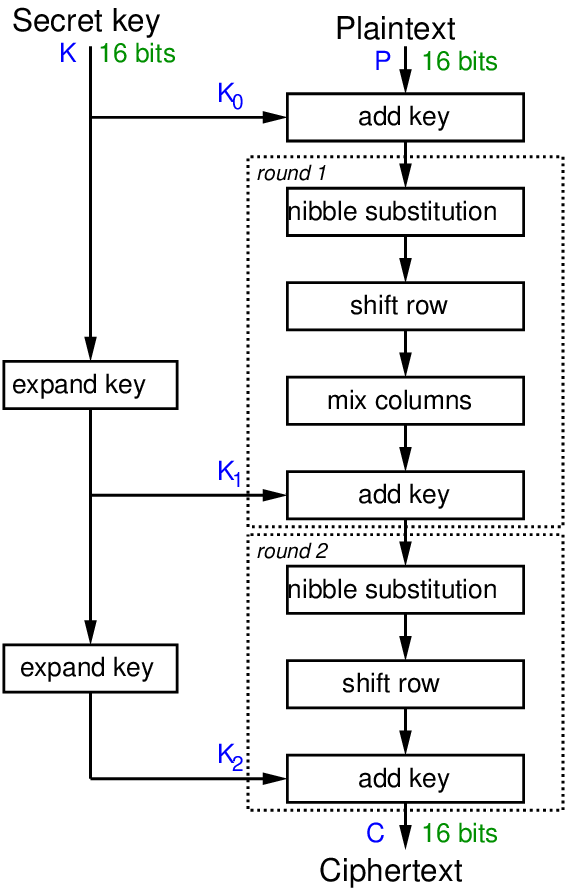
\includegraphics[width=0.5\linewidth]{saes/saes-encryption.png}
    \caption{SAES encryption \cite{Gordon}}
    \label{fig:saes-encryption}
\end{figure}


\subsection{Sub Nibbles}
The sub nibbles operation takes a nibble as input and gives a nibble as output. The Sbox is computed as follows for an input $x$
\begin{enumerate}
    \item Compute the multiplicative inverse $x$ i.e. $y = x^{-1}$ in $GF(2^4)$.
    \item The result of the Sbox is computed using the follows operation:
    
    \begin{equation}\label{eq:sn}
        \begin{bmatrix}
        z_0\\
        z_1\\ 
        z_2\\
        z_3
        \end{bmatrix} = 
        \begin{bmatrix}
        1 & 0 & 1 & 1\\
        1 & 1 & 0 & 1 \\
        1 & 1 & 1 & 0 \\
        0 & 1 & 1 & 1
        \end{bmatrix} 
        \begin{bmatrix}
        y_0 \\ y_1\\
        y_2 \\ y_3
        \end{bmatrix} 
        \oplus
        \begin{bmatrix}
        1  \\ 0\\
        0 \\ 1
        \end{bmatrix} 
    \end{equation}
\end{enumerate}

The final Sbox is the given below:
\begin{center}
\begin{tabular}{ |c|c|c|c|c|c|c|c|c|c|c|c|c|c|c|c|c| } 
 \hline
 $x$ & 0 & 1& 2& 3& 4& 5& 6& 7& 8& 9& A& B& C& D& E& F \\ \hline
 $Sbox(x)$ & 9& 4& A& B& D& 1& 8& 5& 6& 2& 0& 3& C& E& F& 7 \\ \hline
\end{tabular}
\end{center}

\subsection{Shift Rows}
The Shift Rows operation is the same as AES.

\[
    \begin{bmatrix}
    S_0 & S_2\\
    S_1 & S_3
    \end{bmatrix} \longrightarrow
    \begin{bmatrix}
    S_0 & S_2\\
    S_3 & S_1
    \end{bmatrix} 
\]

\subsection{Mix Columns}
SAES work on the ring $\mathbb{F}_2[x]/(x^4 + x +  1)$ and Mix Columns treats 1 byte (1 column of the state matrix) as an element in $GF(2^4)$ with ring $\mathbb{F}_{2^4}[x]/(x^2 + 1)$. The transformation is as follows:

\[
    \begin{bmatrix}
    S_0'\\
    S_1'\\ 
    \end{bmatrix} = 
    \begin{bmatrix}
    1 & 4 \\
    4 & 1 
    \end{bmatrix}
    \begin{bmatrix}
    S_0\\
    S_1\\ 
    \end{bmatrix}
\]
The elements of the matrix are in $\mathbb{F}_{2^4}[x]/(x^2 + 1)$.

\subsection{Key Expansion}
The master key (16 bit) can be thought as 2 bytes $B_0B_1$. SAES uses 3 keys in one full encryption. The first key is the master key. The first round key $B_2B_3$ and the second round key $B_4B_5$ are expanded from the master key using the following algorithm:


\begin{codebox}
\Procname{$\proc{Key Expansion for SAES}(K)$}\label{proc:ke}
\li $\id{keys} \gets [B_0,B_1,B_2,B_3,B_4,B_5]$
\li $keys[0] = K[0 \dots 8]$
\li $keys[1] = K[8 \dots 16]$
\li  \For $i \gets 2$ \To $5$
\li     \Do
                \If $i\%2 == 0$
\li                 \Then
                        $keys[i] = keys[i-2] \oplus RCON(i/2) \oplus Sbox(RotNib(keys[i-1]))$
\li                \Else
\li                    $keys[i] = keys[i-2]\oplus keys[i-1]$
                    \End
        \End
\li \Return $B_0B_1, B_2B_3, B_4B_5$
\end{codebox}

The $RotNib$ function rotates the two nibbles of a byte. $RCON$ is the round constant function and is defined as

\[
    RCON(i) = (x^{i+2} || 0000)
\]

For example $RCON(1) = 10000000$, $RCON(2) = 00110000$.

\section{Quantum SAES18}\label{sec:qsaes18}

We now describe the design of the quantum circuit for SAES as proposed by \cite{Almazrooie} and call it QSAES18 as it was published in the year 2018. The proposed design is shown in Figure \ref{fig:qaes18}. PTXT denotes plaintext, SN denotes sub nibbles, MC denotes mix columns and RC denotes round constant. Initially, key is added to the first 16 qubits followed by the addition of plaintext. 

\begin{figure}[h!]
    \centering
    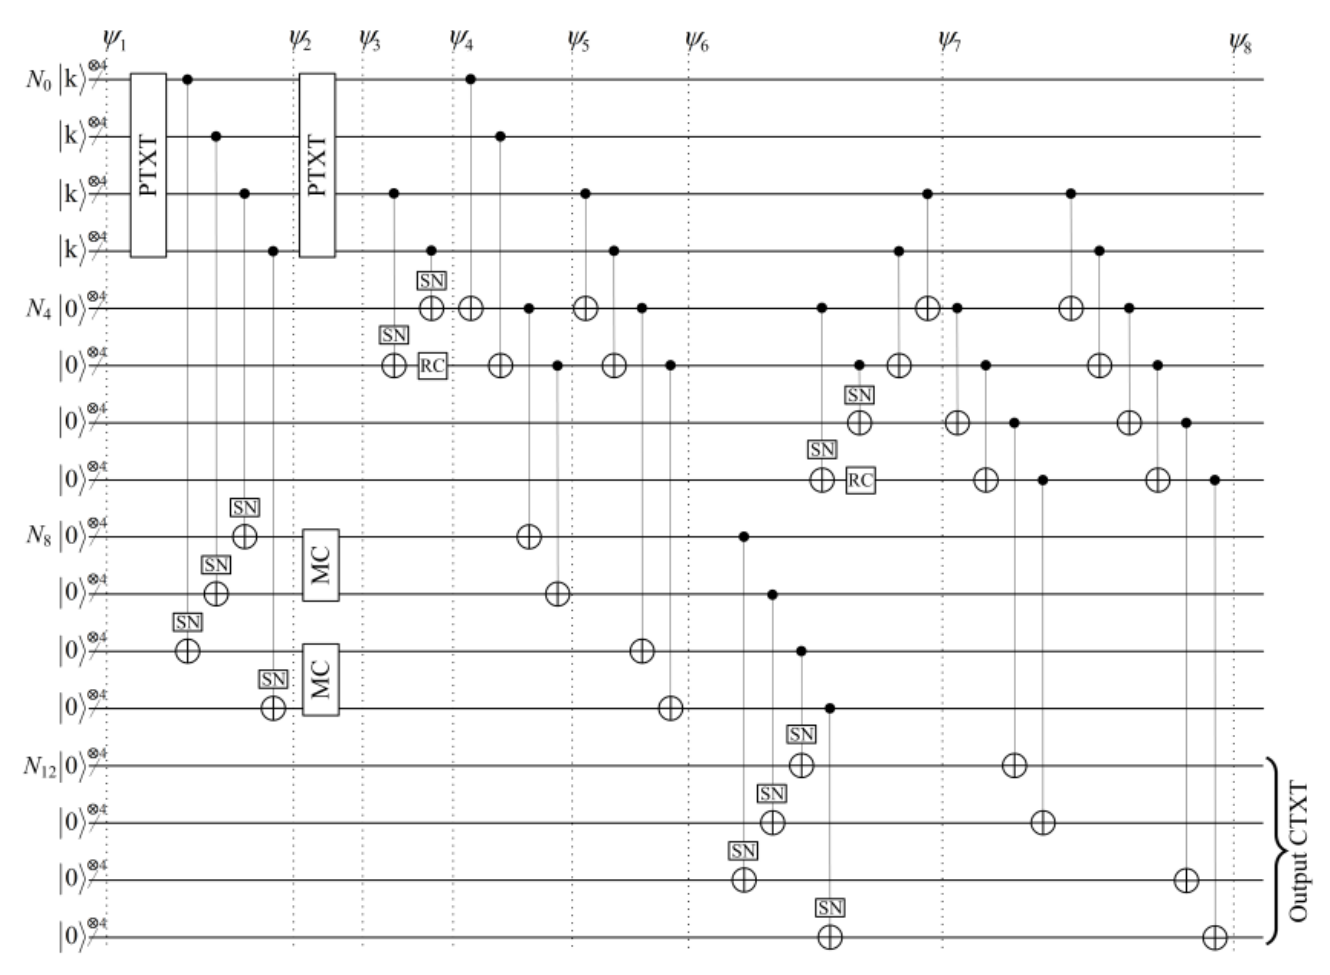
\includegraphics[width=\linewidth]{saes18/qsaes18.png}
    \caption{QSAES18 \cite{Almazrooie}}
    \label{fig:qaes18}
\end{figure}

\subsection{Working of the circuit}
We briefly describe the working of the quantum circuit. $\ket{\psi_i}$ denote the state at a slice in the circuit.

\subsubsection{Initialisation}
At state $\ket{\psi_1}$, the qubits are initialized with the master key and then XORed with the plaintext.

\subsubsection{Round 1}

The first four nibbles are passed through the Sbox for the sub-nibbles operation. For the shift row operation, they are mapped to other nibbles. Specifically

\begin{align*}
    N_0 &\longrightarrow N_{10} \\
    N_1 &\longrightarrow N_9  \\
    N_2 &\longrightarrow N_8 \\
    N_3 &\longrightarrow N_{11}
\end{align*}

\[
    \begin{bmatrix}
    S_0 & S_2\\
    S_1 & S_3
    \end{bmatrix} \longrightarrow
    \begin{bmatrix}
    S_0 & S_2\\
    S_3 & S_1
    \end{bmatrix} 
\]
The state after shift rows is at $\ket{\psi_2}$. Note that the plaintext is again XORed with the first 4 nibbles at $\ket{\psi_2}$ to recover the master key.
 
After the shift rows operation, mix columns will operate on the the two columns $\begin{bmatrix}
S_0\\ S_3
\end{bmatrix}$ and $\begin{bmatrix}
S_2 \\ S_1
\end{bmatrix}$. $S_0, S_3$ are on nibble $N_{10}, N_{11}$ and $S_2, S_1$ are on nibble $N_8, N_9$. Therefore the two mix column gates are placed accordingly. 


\subsubsection{Round 2}
Similar to round 1, the state after sub nibbles and shift rows is at $\ket{\psi_7}$. The key expansion part is continued by the top qubits and follows the same method as explained previously. The final ciphertext is captured at $N_{12},N_{13},N_{14},N_{15}$ at state $\ket{\psi_8}$.


We now describe the implementation of each operation

\subsection{Sub Nibbles}

As per equation \ref{eq:sn}, we need to find the multiplicative inverse of the input $x$. The authors use the Fermat inversion algorithm which is the square and multiply method to find multiplicative inverse in $GF(2^4)$. The theorem states that the multiplicative inverse of an element $x \in GF(2^4)$ can be calculated as follows:

\begin{equation*}
    x^{-1} = x^{2^4 - 2} = x^{16-2} = x^{14} = x^{2} \times (x^{2})^{2} \times ((x^{2})^{2})^{2}
\end{equation*}

The above equation has 2 multiplication operations and 3 squaring operations. The authors use a quantum multiplier in $GF(2^4)$ from \cite{Cheung}. The quantum circuit for the multiplier is shown in Figure \ref{fig:mul}. 


\begin{figure}[h!]
    \centering
    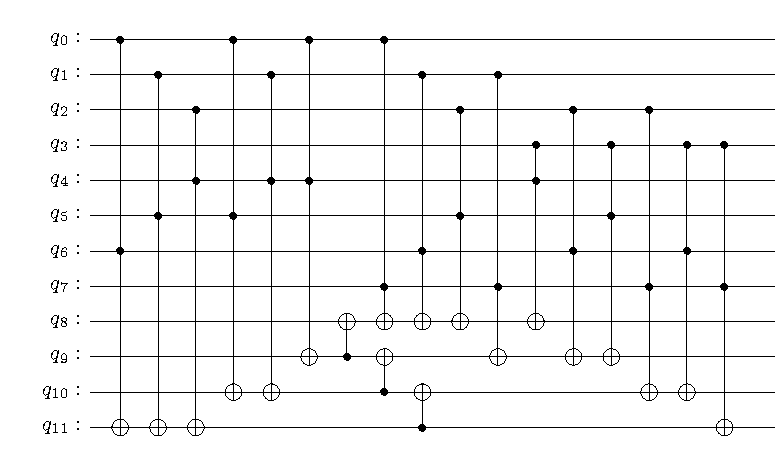
\includegraphics[width=\linewidth]{saes18/multiplier.pdf}
    \caption{Multiplier}
    \label{fig:mul}
\end{figure}

The first 8 qubits are input to the multiplier circuit. $q_0 - q_3$ is the first vector and $q_4 - q_7$ is the second vector. The output is taken at the last 4 qubits $q_8 - q_{11}$.

The squarer circuit can be expressed by using the following equation for some input $x$.

\begin{equation}\label{eq:sq}
    \begin{bmatrix}
    y_0\\
    y_1\\ 
    y_2\\
    y_3
    \end{bmatrix} = 
    \begin{bmatrix}
    1 & 0 & 1 & 0\\
    0 & 0 & 1 & 0 \\
    0 & 1 & 0 & 1 \\
    0 & 0 & 0 & 1
    \end{bmatrix} 
    \begin{bmatrix}
    x_0 \\ x_1\\
    x_2 \\ x_3
    \end{bmatrix}
\end{equation}

For the squarer circuit, the authors use the CNOT synthesis algorithm to decompose the matrix of equation \ref{eq:sq}. The squarer circuit is shown in Figure \ref{fig:sq}.

\begin{figure}[h!]
    \centering
    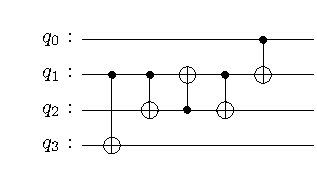
\includegraphics[width=0.5\linewidth]{saes18/squarer.pdf}
    \caption{Squarer}
    \label{fig:sq}
\end{figure}

For the affine transformation (equation \ref{eq:sn}), the affine matrix is decomposed to remove the need for ancilla qubits. Figure \ref{fig:aff} shows the circuit for affine transformation.

\begin{figure}[h!]
    \centering
    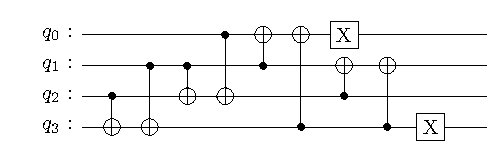
\includegraphics[width=0.8\linewidth]{saes18/affine.pdf}
    \caption{Affine transformation}
    \label{fig:aff}
\end{figure}

The complete Sbox circuit is shown in Figure \ref{fig:sb}. The input is taken from the first 4 qubits and the output is taken at the last 4 qubits. 8 ancilla qubits are used.


\begin{figure}[h!]
    \centering
    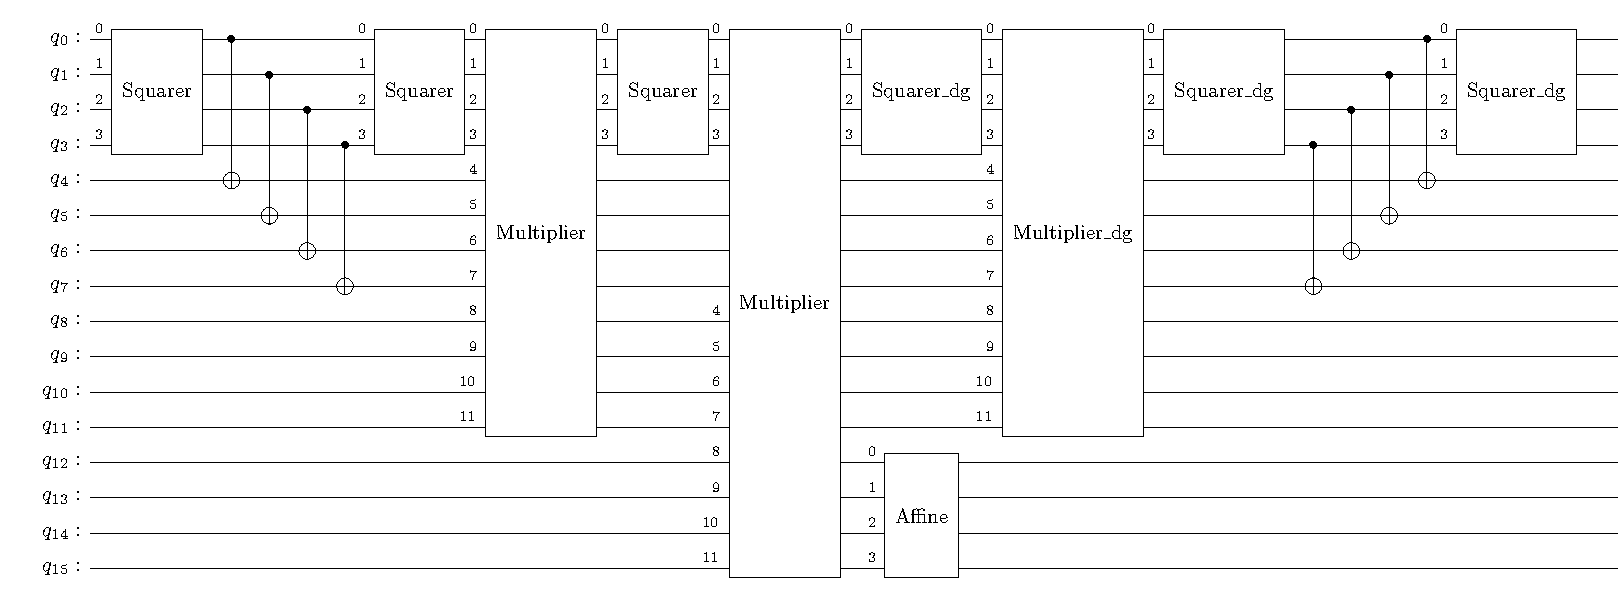
\includegraphics[width=1\linewidth]{saes18/sbox.pdf}
    \caption{Sbox}
    \label{fig:sb}
\end{figure}ff


\subsection{Mix columns}
CNOT synthesis algorithm is used to remove the need for ancilla qubits by decomposing the mix column matrix. Figure \ref{fig:mc} shows the circuit for mix column.

\begin{figure}[h!]o
    \centering
    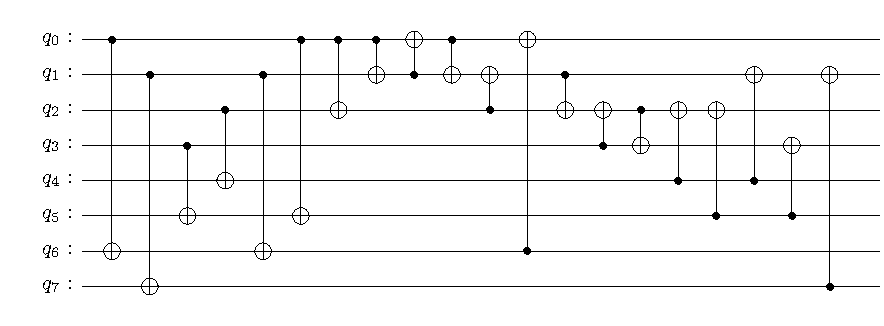
\includegraphics[width=1\linewidth]{saes18/mc.pdf}
    \caption{Mix column}
    \label{fig:mc}
\end{figure}

The circuit takes 1 byte (1 column of the state matrix) and outputs the corresponding matrix multiplication in $GF(2^4)$.


\subsection{Round Constants}

\subsection{Complexity Analysis}
The work was focused on reducing the number of qubits and since the number of gates used is inversely proportional to the number of qubits, the circuit depth is bound to increase. Still, the quantum circuit uses a polynomial number of gates. The cost for implementing SAES is shown in Table \ref{tab:cost}:
\begin{center}
\begin{table}[h!]
    \centering
    \begin{tabular}{ |c|c|c|c|c|c| } 
     \hline
       & Qubits & X & CX & CCX & Ancilla \\ \hline
     Key expansion & 32 & 10& 568 & 192 & 8 \\ \hline
     Encryption & 32 & 16 & 512 & 384 & - \\ \hline
     Total & 64 & 26 & 1080 & 576 & 8 \\ \hline
    \end{tabular}
    \caption{Cost for QSAES18 \cite{Almazrooie}}
    \label{tab:cost}
\end{table}
\end{center}

\subsection{Grover's Attack}
To perform Grover's attack, a reversible circuit of the block cipher is needed. The circuit shown in Figure \ref{fig:qaes18} is only for encryption. To create a reversible circuit, all the operations need to be implemented in reverse order. This will double the cost of Table \ref{tab:cost}. The boolean function for Grover's oracle can be defined as follows:

\begin{equation*}
 f(k) = 
 \begin{cases} 
      1 & SAES(k, p) = c\\
      0 & else 
  \end{cases}
\end{equation*}

$k$ is the key which encrypts $p$ to $c$ using $SAES$ encryption oracle. Figure \ref{fig:grov18} shows the one iteration of Grover's attack on SAES. At $\ket{\psi_1}$, we have all the qubits in a superposition state which describes all possible keys. The encryption is completed at $\ket{\psi_2}$ and if the ciphertext obtained from the oracle matches with the actual ciphertext, then the target qubit (oracle qubit in the figure) is flipped (this logic is implemented by placing the actual ciphertext in after the encryption oracle and flipping the oracle qubit using unbounded Toffoli gate \cite{mcmt}). At $\ket{\psi_3}$ we complete the reversible circuit of SAES and at $\ket{\psi_4}$ we obtain the state after Grover's Diffusion Operator.

\begin{figure}[h!]
    \begin{center}
\begin{quantikz}
\lstick{$\ket{0}^{\otimes 16}$\\key} &[2mm]\gate{H^{\otimes 16}}\slice{$\ket{\psi_1}$} & \gate[wires=2][2cm]{P~SAES} & \qw & \qw \slice{$\ket{\psi_2}$}& \qw & \gate[wires=2][2cm]{P~SAES^\dagger}\slice{$\ket{\psi_3}$} & \gate{INV}\slice{$\ket{\psi_4}$} & \qw \\
\lstick{$\ket{0}^{\otimes 63}$\\work space} &[2mm] \qw & & \gate{C} & \ctrl{1} & \gate{C} & & \qw & \qw \\
\lstick{$\ket{0}$\\oracle} &[2mm] \gate{X} & \gate{H} & \qw & \targ{} & \qw & \qw & \qw & \qw 
\end{quantikz}
\end{center}
    \caption{Grover's Attack on SAES}
    \label{fig:grov18}
\end{figure}

To calculate the number of iterations required for a successful Grover's Attack, we use the following equation:
\begin{equation}
    t = \frac{\pi}{4}\sqrt{\frac{2^k}{s}}
\end{equation}

$k$ is the size of the key and therefore $2^k$ is the total key space. $s$ is the total number of solutions possible. More than one key can encrypt the same plaintext to the same ciphertext. The authors chose $r = 2$, where $r$ is the number of plaintext-ciphertext pairs. This guarantees to find the unique key. Plugging the values we get:

\begin{equation*}
    t = \frac{\pi}{4}\sqrt{\frac{2^{16}}{2}} = 142
\end{equation*}

They propose a modified version of Grover's Attack to find the unique key which is shown in Figure \ref{fig:grov18u}.


\begin{figure}[h!]
    
    \resizebox{15cm}{!}{
    \begin{quantikz}
    \lstick{$\ket{0}^{\otimes 16}$\\key} &[2mm]\gate{H^{\otimes 16}} & \gate[wires=2][2cm]{P_1~SAES} & \qw & \qw & \qw & \gate[wires=2][2cm]{P_1~SAES^\dagger} & \gate[wires=2][2cm]{P_2~SAES} & \qw & \qw &\qw & \gate[wires=2][2cm]{P_2~SAES^\dagger}& \gate[wires=2][2cm]{P_1~SAES} & \qw & \qw & \qw & \gate[wires=2][2cm]{P_1~SAES^\dagger} & \gate{INV} & \qw \\
    \lstick{$\ket{0}^{\otimes 63}$\\work space} &[2mm] \qw & & \gate{C_1} & \ctrl{1} & \gate{C_1} & & \qw & \gate{C_2} & \ctrl{2} & \gate{C_2} &\qw &\qw & \gate{C_1} & \ctrl{1} & \gate{C_1} & \qw & \qw & \qw  \\
    \lstick{$\ket{0}$\\oracle} &[2mm]  \qw & \qw & \qw &\targ{}&  \qw & \qw & \qw  & \qw& \control{} & \qw & \qw & \qw & \qw &\targ{}  &  \qw &  \qw &  \qw & \qw   \\
    \lstick{$\ket{0}$\\oracle} &[2mm] \gate{X} & \gate{H} & \qw & \qw & \qw & \qw  & \qw & \qw &\targ{} & \qw & \qw & \qw & \qw & \qw & \qw & \qw &\qw &\qw
    \end{quantikz}
    }
    
    \caption{Grover's Attack to find unique key with r = 2}
    \label{fig:grov18u}
\end{figure}

The corresponding boolean function is described as follows:
\begin{equation*}
 f(k) = 
 \begin{cases} 
      1 & (SAES(k, p_1) = c_1) \wedge (SAES(k, p_2) = c_2) \\
      0 & else 
  \end{cases}
\end{equation*}

Using the circuit shown in Figure \ref{fig:grov18u}, the authors were able to successfully run Grover's Attack on SAES. For the plaintext 0110 1111 0110 1011 and ciphertext 0000 0111 0011 1000, the actual key is 1010 0111 0011 1011. We verified this classically using a python program \cite{Gopal}.

\section{Quantum SAES21}\label{sec:qsaes21}
We now describe the design of the quantum circuit for SAES as proposed by \cite{Jang} and call it QSAES21 as it was published in the year 2021. This version is optimized compared to \cite{Almazrooie} as it only uses 32 qubits and no ancilla qubits. The proposed design is shown in Figure \ref{fig:qsaes21}. 

\begin{figure}[h!]
    \centering
    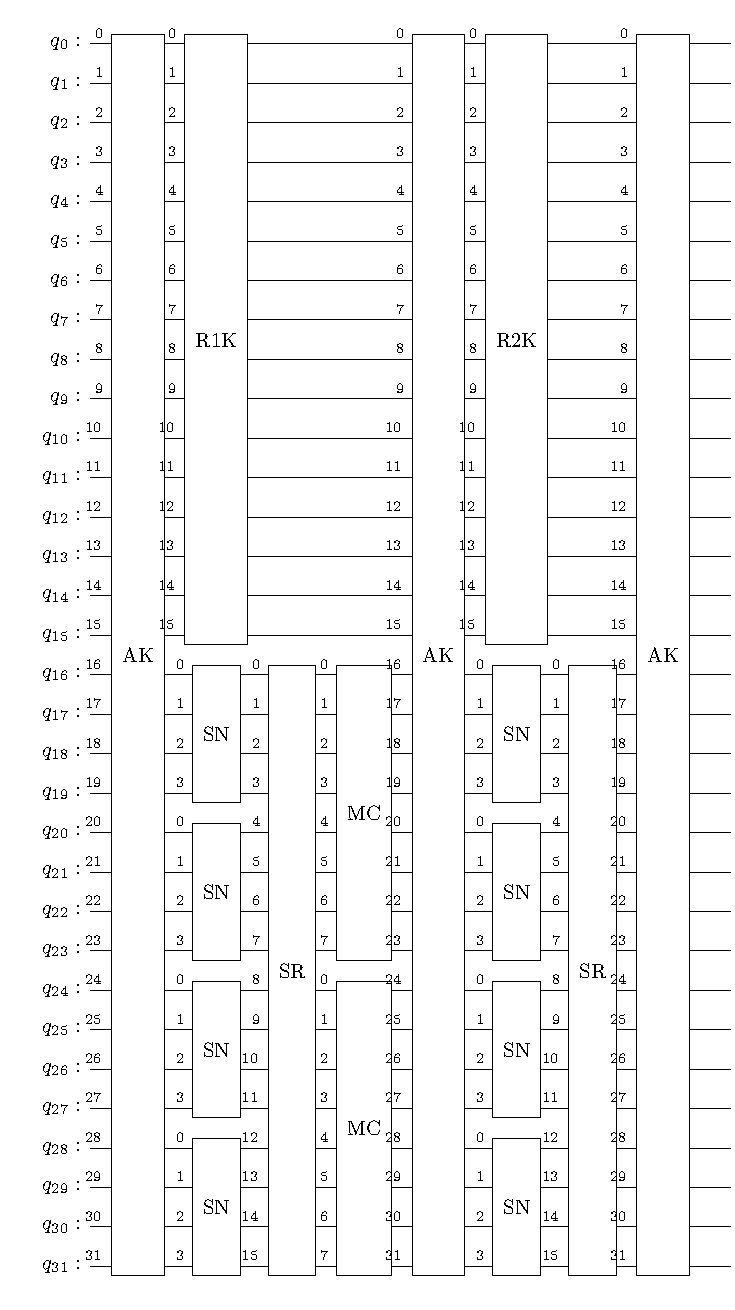
\includegraphics[width=0.7\linewidth]{saes21/saes.pdf}
    \caption{QSAES21}
    \label{fig:qsaes21}
\end{figure}

The top 16 qubits are used for storing the master key and for the process of key expansion. The bottom 16 qubits are used for storing plaintext, round operations, and outputting ciphertext.

\subsection{Sub Nibbles}
Unlike \cite{Almazrooie} which uses 16 qubits (4 input, 4 output, and 8 ancillae) for Sbox computation, \cite{Jang} uses only 4 qubits using LIGHTER-R tool \cite{LighterR}. The output of the quantum circuit is a permutation of the bits of the actual Sbox output and therefore SWAP gates are used which are not measured in the overall quantum resources used in QSAES21. Figure \ref{fig:sb21} shows the quantum circuit for Sbox.

\begin{figure}[h!]
    \centering
    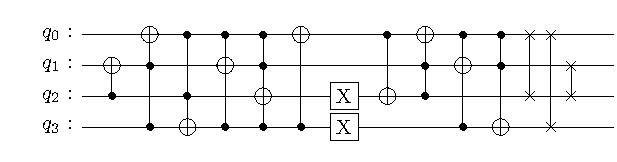
\includegraphics[width=1\linewidth]{saes21/sbox.pdf}
    \caption{Sbox}
    \label{fig:sb21}
\end{figure}

We also need to implement the inverse Sbox operation which will be required during reversible SAES. Figure \ref{fig:isb21} shows the quantum circuit of inverse Sbox.

\begin{figure}[h!]
    \centering
    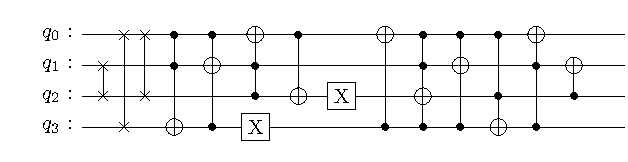
\includegraphics[width=1\linewidth]{saes21/inv_sbox.pdf}
    \caption{Inverse Sbox}
    \label{fig:isb21}
\end{figure}

\subsection{Mix Columns}

Similar to \cite{Almazrooie}, the authors use 8 qubits to perform mix columns operation on 1 column of the state matrix. Figure \ref{fig:mc21} shows the quantum circuit for mix column operation on 1 byte (1 column) of the state matrix. Compared to \cite{Almazrooie}, the authors use less number of qubits but require SWAP gates to get the correct result. Since SWAP gates are not counted in the quantum resources, the quantum circuit for the mix column by \cite{Jang} is more optimal compared to \cite{Almazrooie}.


\begin{figure}[h!]
    \centering
    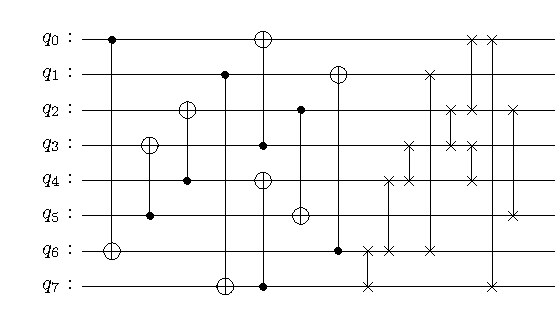
\includegraphics[width=0.7\linewidth]{saes21/mc.pdf}
    \caption{Mix column}
    \label{fig:mc21}
\end{figure}

\subsection{Shift Rows}
The authors implemented shift rows operation using swap gates only whereas \cite{Almazrooie} used extra qubits for that with additional CNOT gates. The circuit for shift rows is shown in Figure \ref{fig:sr21}.

\begin{figure}[h!]
\centering
\begin{subfigure}{.5\textwidth}
  \centering
  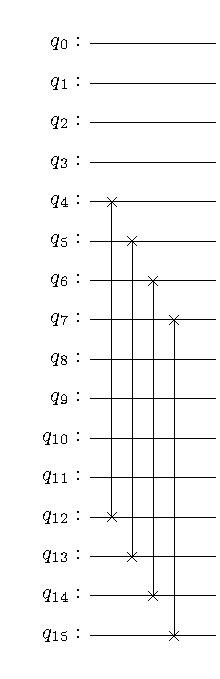
\includegraphics[width=0.3\linewidth]{saes21/sr.pdf}
  \caption{Shift rows}
  \label{fig:sr21}
\end{subfigure}%
\begin{subfigure}{.5\textwidth}
  \centering
  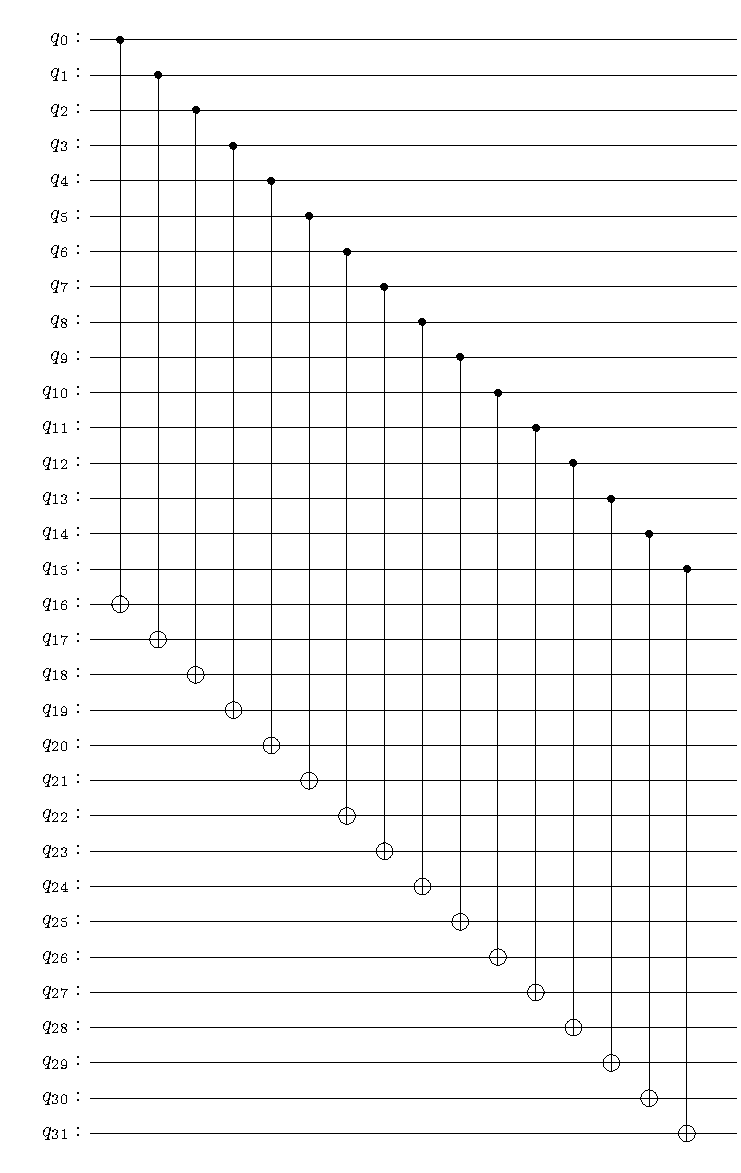
\includegraphics[width=0.6\linewidth]{saes21/ark.pdf}
  \caption{Add round key}
  \label{fig:ark21}
\end{subfigure}
\caption{Shift rows and Add round key}
\label{fig:test}
\end{figure}

\subsection{Add Round Key}
Add round key can be implemented simply using 16 CNOT gates as shown in Figure \ref{fig:ark21}

\subsection{Key Expansion}
Round keys are generated on the fly. Figure \ref{fig:rk121} shows the circuit for generating the first round key from the master key. 

\begin{figure}[h!]
    \centering
    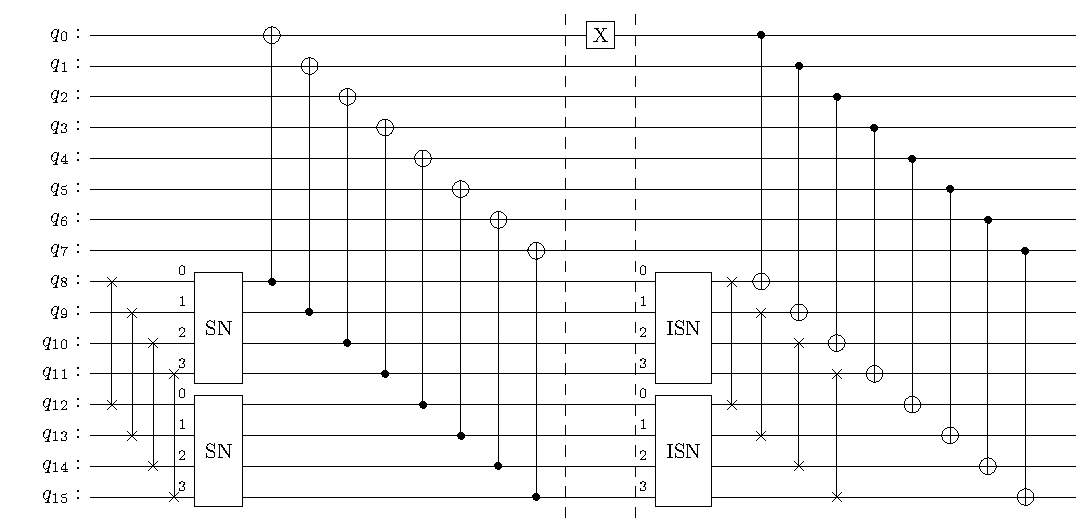
\includegraphics[width=0.8\linewidth]{saes21/r1k.pdf}
    \caption{Round key 1}
    \label{fig:rk121}
\end{figure}

Referring to the key expansion algorithm \ref{proc:ke}, for the first round key, we perform swap and substitution of $B_1$ (SWAP gate and Sbox gate) and then xor it with $B_0$ (CNOT gates). Then xor is performed with the round constant (single not gate as the first round key is 10000000). Now the first 8 qubits hold $B_2$. To get $B_3$, we need to xor $B_1$ and $B_2$. Since the operations on the bottom 8 qubits result in the loss of $B_1$, we need to perform inverse swap and substitution on the lower 8 qubits to get back $B_1$. Then we XORed $B_2$ with $B_1$ to get $B_3$. 

Therefore the top 8 qubits hold $B_2$ and the bottom 8 qubits hold $B_3$.

Similarly Figure \ref{fig:rk221} shows the circuit for generating the second round key with round constant as 01100000.

\begin{figure}[h!]
    \centering
    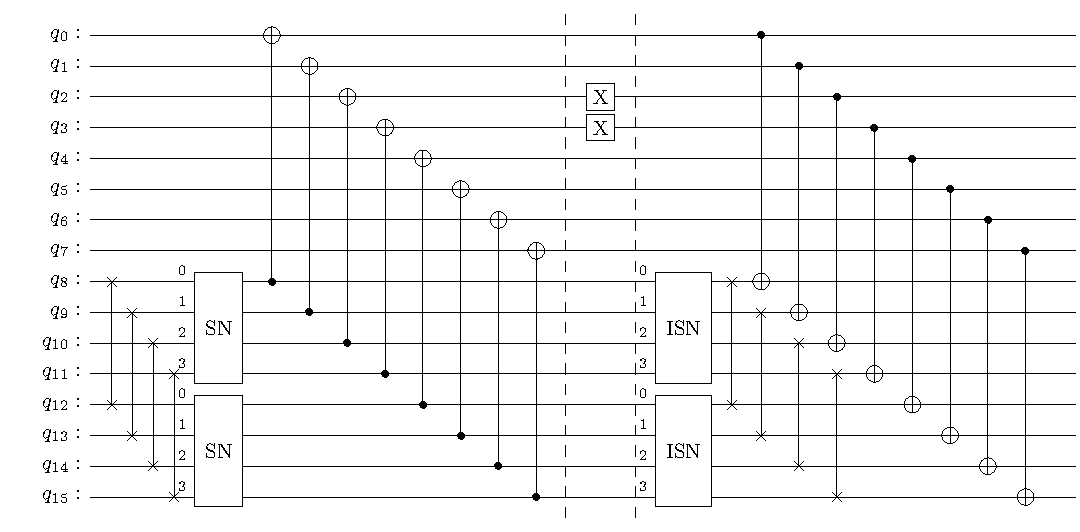
\includegraphics[width=0.8\linewidth]{saes21/r2k.pdf}
    \caption{Round key 2}
    \label{fig:rk221}
\end{figure}

\subsection{Evaluation}

In all the experiments performed, the quantum circuit was transpiled with an optimization level 2. According to Qiskit docs, transpilation is the process of rewriting a given input circuit to match the topology of a specific quantum device, and/or to optimize the circuit for execution on present-day noisy quantum systems \cite{transpile}. The optimization level defines how much optimization to perform on the circuits. Higher levels generate more optimized circuits, at the expense of longer transpilation time. * 0: no optimization * 1: light optimization * 2: heavy optimization * 3: even heavier optimization.  \cite{transpile}

\begin{figure}[h!]
    \centering
    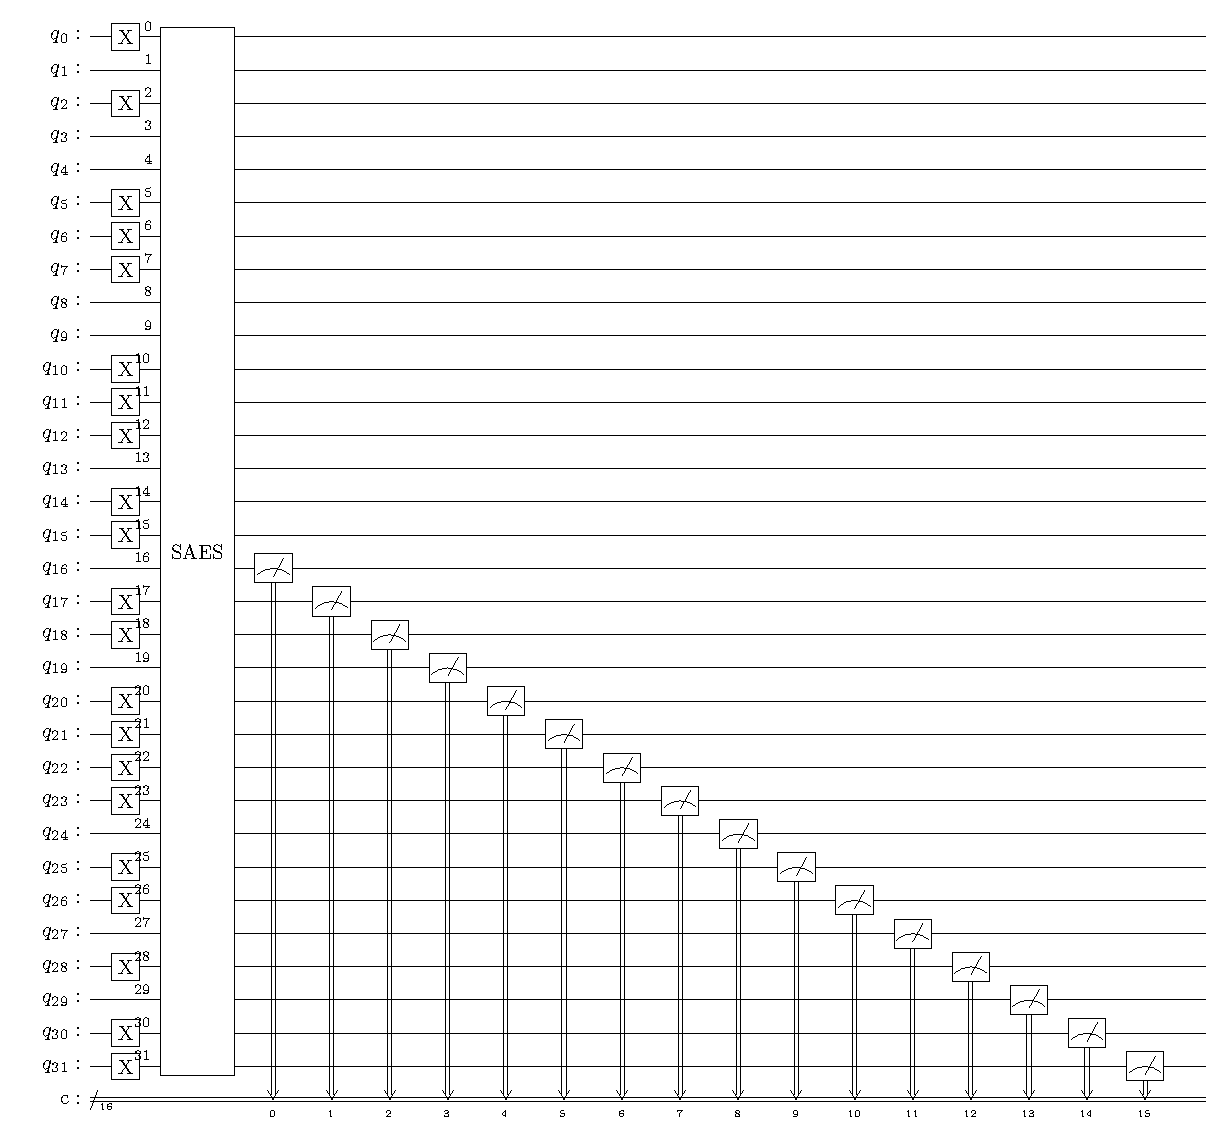
\includegraphics[width=0.8\linewidth]{saes21/expt1.pdf}
    \caption{Verification of QSAES21}
    \label{fig:expt1}
\end{figure}


\subsubsection{Experiment 1}
In this experiment, we checked whether the quantum circuit for QSAES21 gives the same output as its classical counterpart. Figure \ref{fig:expt1} shows the circuit in which we initialize the qubits with a key 1010 0111 0011 1011 and plaintext 0110 1111 0110 1011 and obtained the ciphertext 0000 0111 0011 1000 which is the same as given by our implementation of the classical algorithm \cite{Gopal}. The simulation was performed on IBMQ QASM Simulator \cite{IBMQ} and the results can be found at \cite{Gopal}. Figure \ref{fig:expt1res} shows the result obtained.

\begin{figure}[h!]
    \centering
    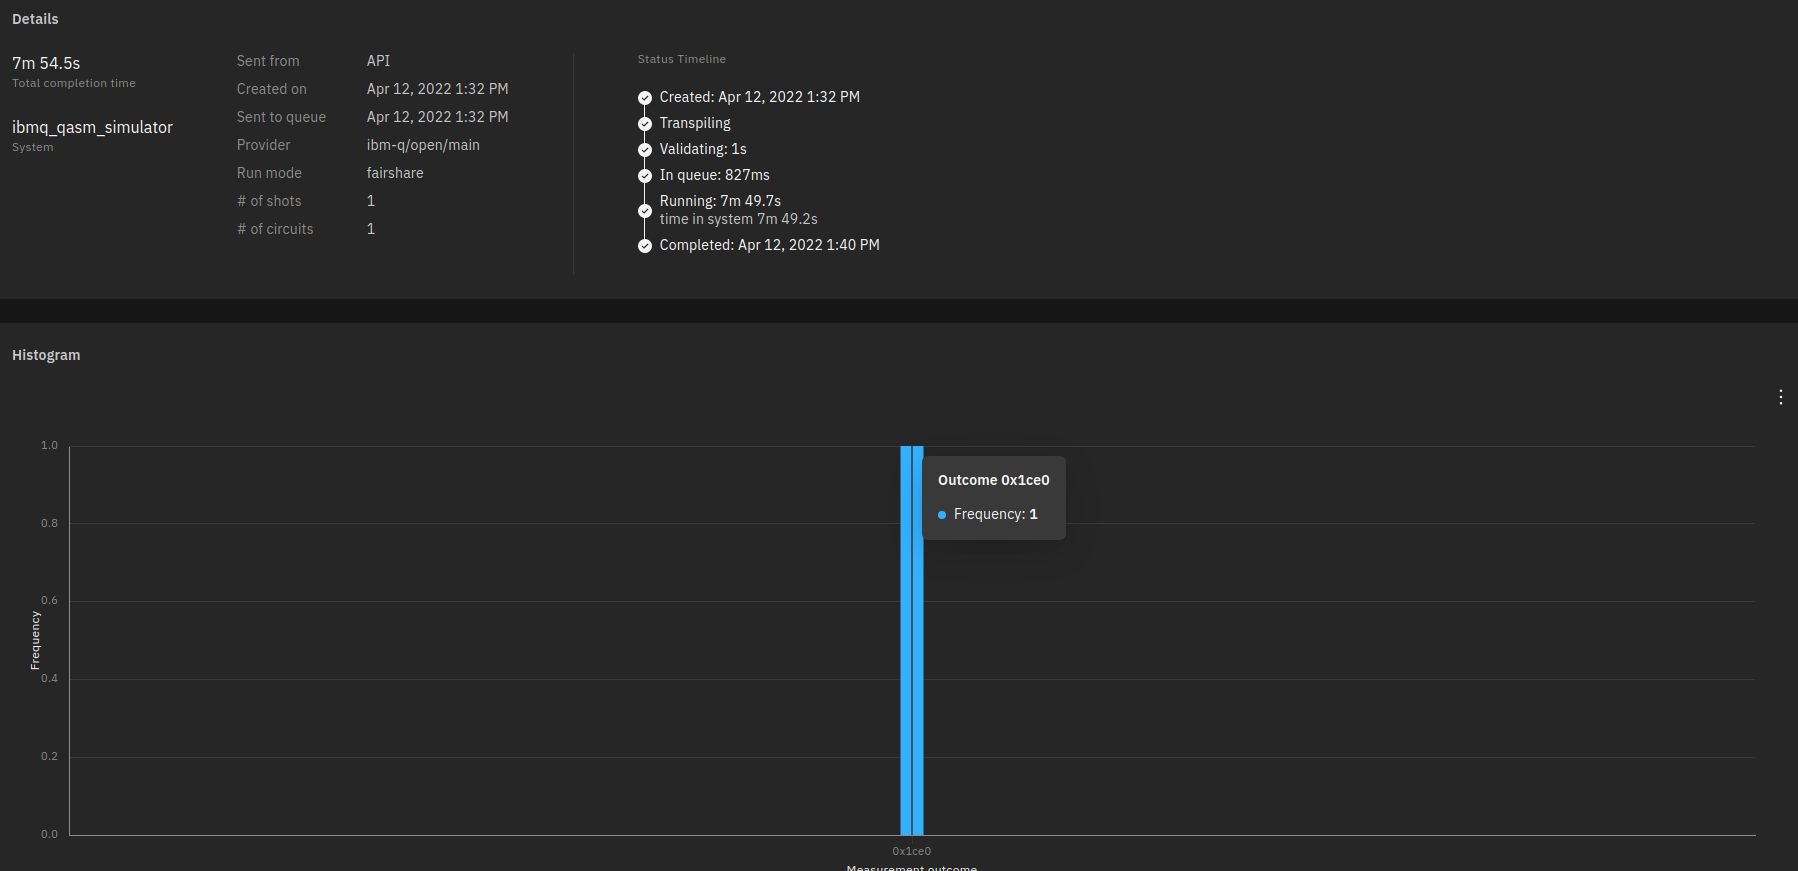
\includegraphics[width=\linewidth]{saes21/encryption.png}
    \caption{Output of encryption of plaintext 0110 1111 0110 1011 with key 1010 0111 0011 1011}
    \label{fig:expt1res}
\end{figure}

We can see that the output is $0x1ce0$ in hexadecimal, which in binary is 0001 1100 1110 0000 which is the reverse of the ciphertext (reverse because Qiskit's \cite{Qiskit} measurement shows the bottom qubit first). 


\subsubsection{Experiment 2}
Figure \ref{fig:expt2} shows the quantum circuit for this experiment performed using IMBQ Statevector simulator \cite{IBMQ}. We put the key in a superposition of all states and fix the plaintext. The state vector simulator gives all possible states in the output. This will result in all possible key, ciphertext pairs. Ideally, we should run for $2^{32}$, but the simulator gave a timeout error. We were able to run it for 4000 shots. Results can be found at \cite{Gopal}.  Figure \ref{fig:expt2res} shows the result obtained.

\begin{figure}[h!]
    \centering
    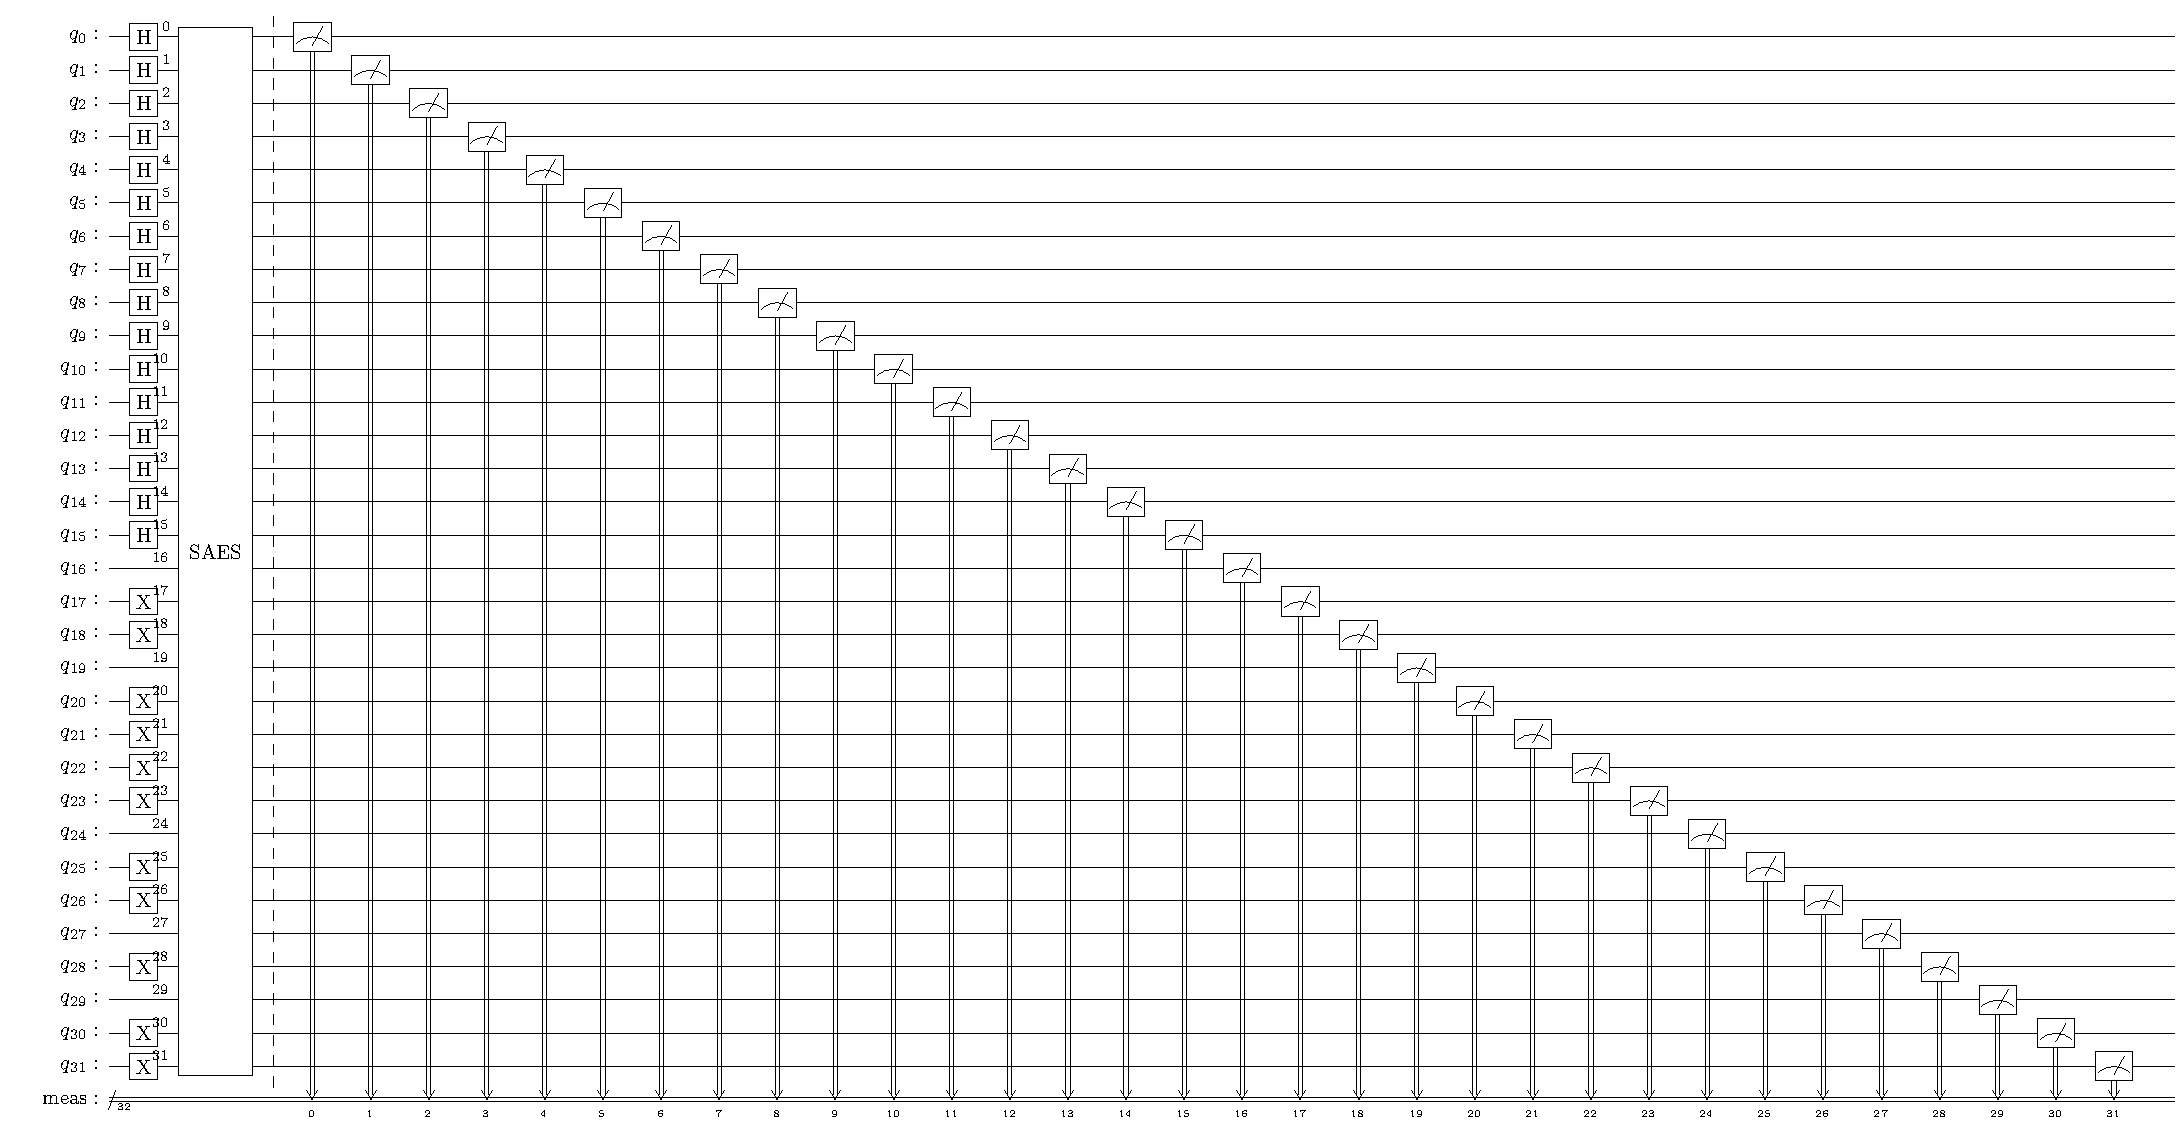
\includegraphics[width=1.1\linewidth]{saes21/expt2.pdf}
    \caption{State vector simulation}
    \label{fig:expt2}
\end{figure}


\begin{figure}[h!]
    \centering
    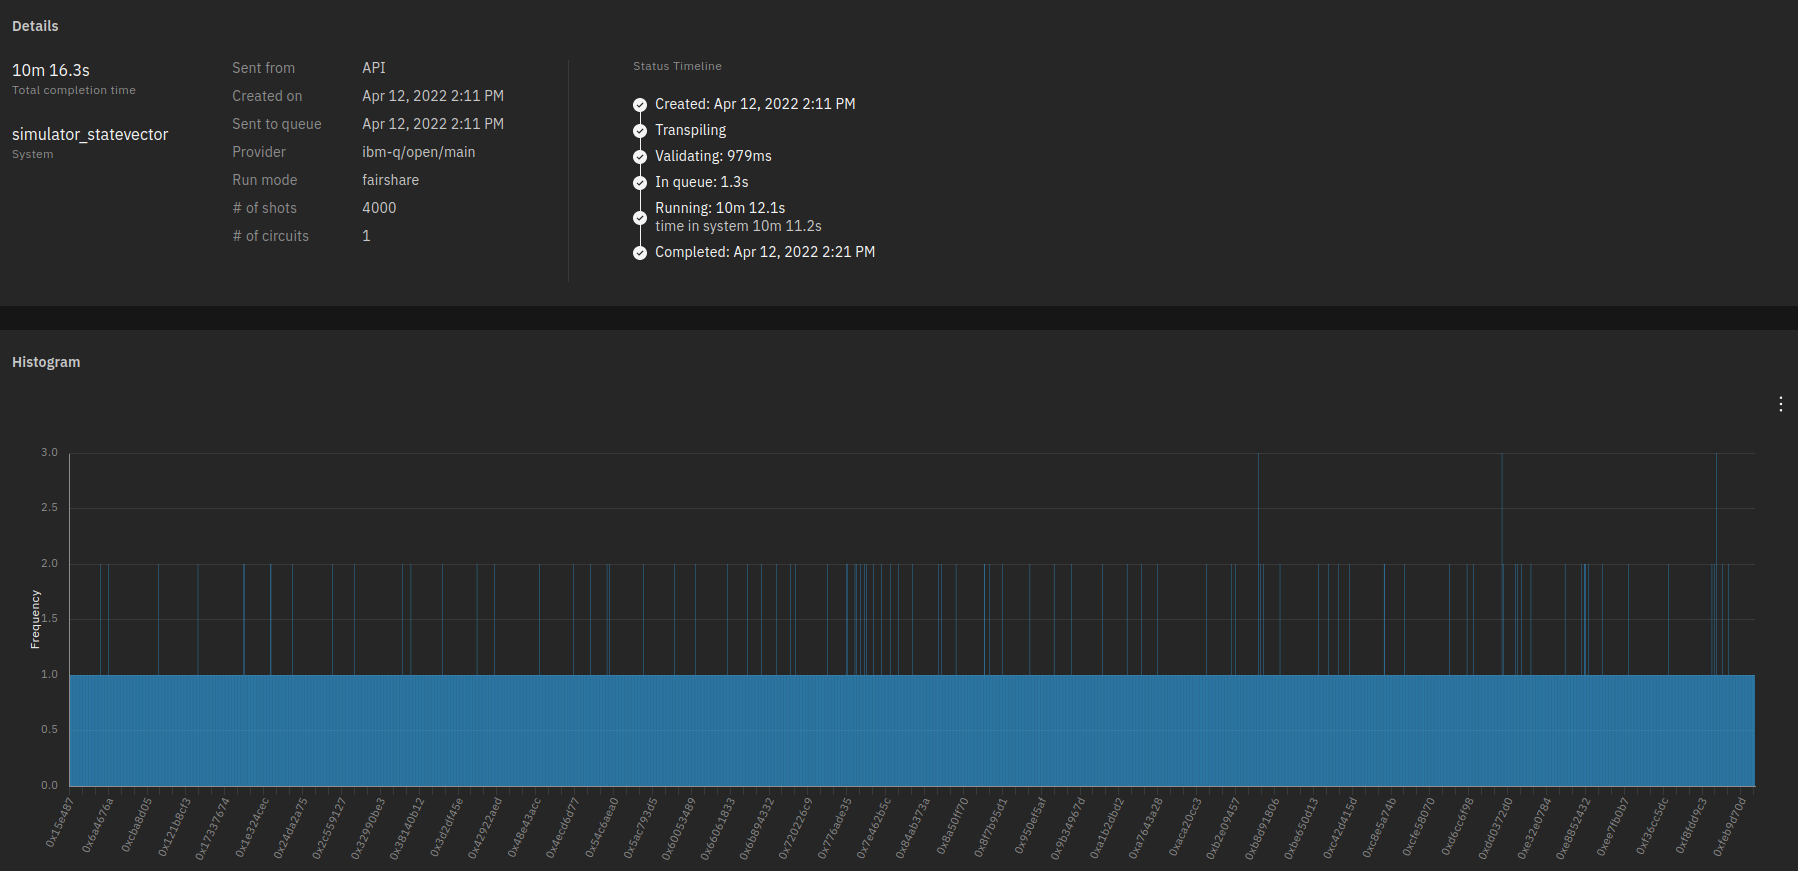
\includegraphics[width=\linewidth]{saes21/statevector.png}
    \caption{Keys in Superposition}
    \label{fig:expt2res}
\end{figure}

We can see that in the output maximum states have frequency 1. Some states have frequencies 2 and even 3. This is possible has the superposition can collapse into any $2^{32}$ states.


\subsubsection{Grover's Attack}
For performing Grover's Attack, we need to create the oracle circuit. Figure \ref{fig:o121} shows the oracle. The plaintext-ciphertext pair used is (0110111101101011, 0000011100111000). The oracle is the same as used by \cite{Almazrooie}. It consists of a SAES encryption circuit followed by the unbounded Toffoli gate \cite{mcmt}. Then the reversible circuit is used to undo the operation of SAES. Using this circuit, Grover's Attack circuit is designed as shown in Figure \ref{fig:grov21}.

Since this will not find the unique key, another oracle is designed in which a different plaintext-ciphertext pair is used (0110111101101011,0000011100111000) whose circuit is shown in Figure \ref{fig:o221}. The modified Grover's Attack circuit is shown in Figure \ref{fig:grov21u} which is similar to Figure \ref{fig:grov18u}.

Table \ref{tab:cost21} compares the work of \cite{Almazrooie} and \cite{Jang}. We can see that the number of gates is reduced significantly.

\begin{figure}[h!]
\centering
\begin{subfigure}{.5\textwidth}
  \centering
  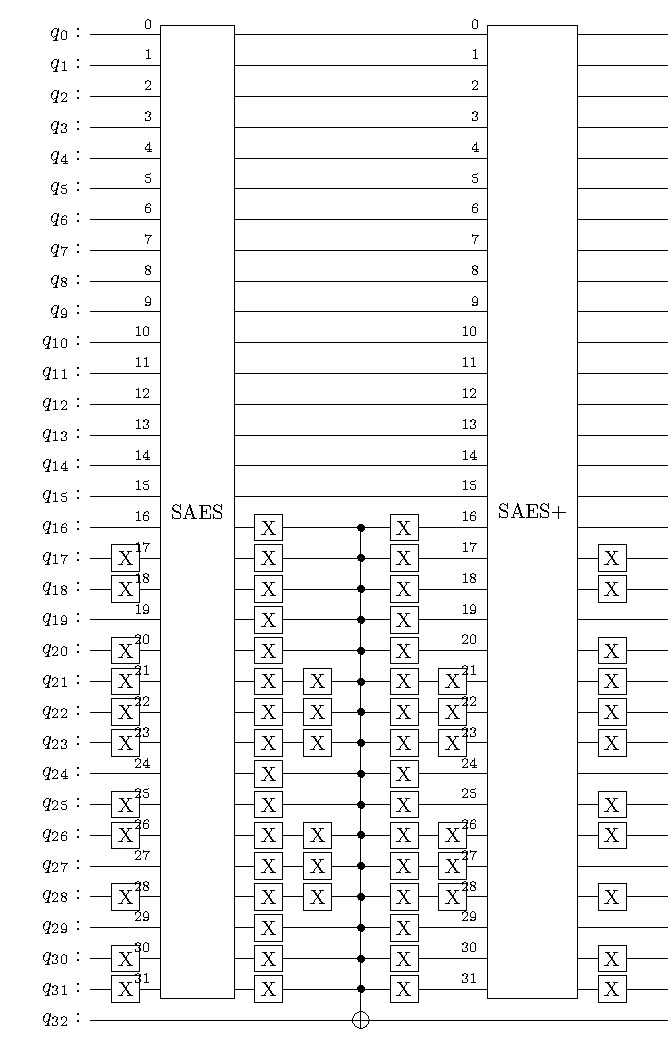
\includegraphics[width=0.8\linewidth]{saes21/Uf1.pdf}
  \caption{Oracle 1}
  \label{fig:o121}
\end{subfigure}%
\begin{subfigure}{.5\textwidth}
  \centering
  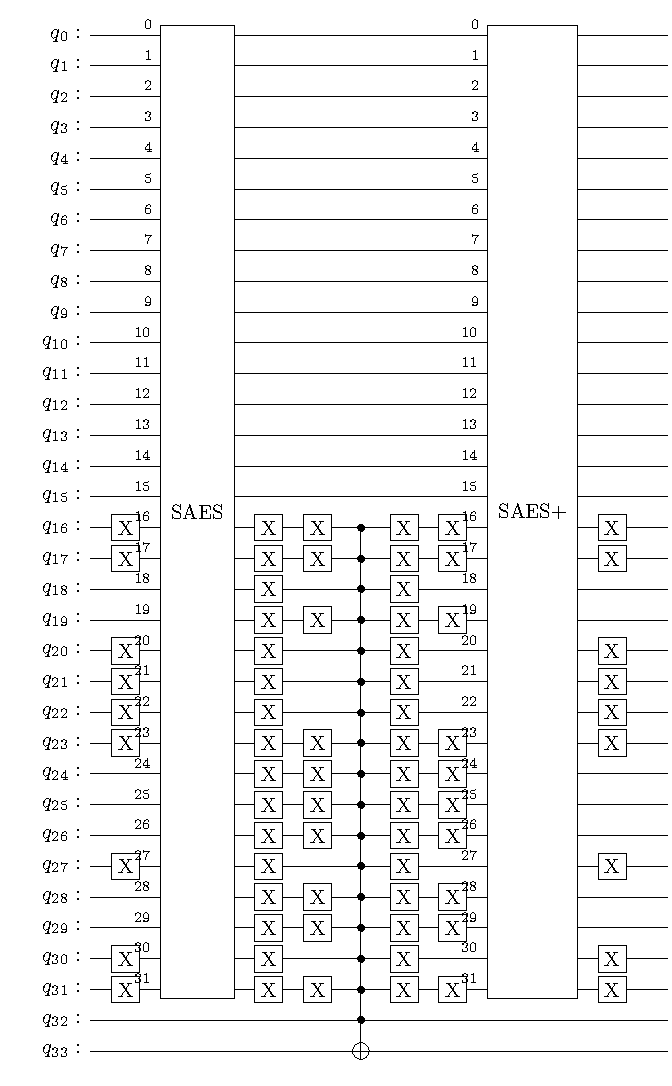
\includegraphics[width=0.8\linewidth]{saes21/Uf2.pdf}
  \caption{Oracle 2}
  \label{fig:o221}
\end{subfigure}
\caption{Oracles for Grover's Attack}
\label{fig:test}
\end{figure}

\begin{figure}[h!]
    \centering
    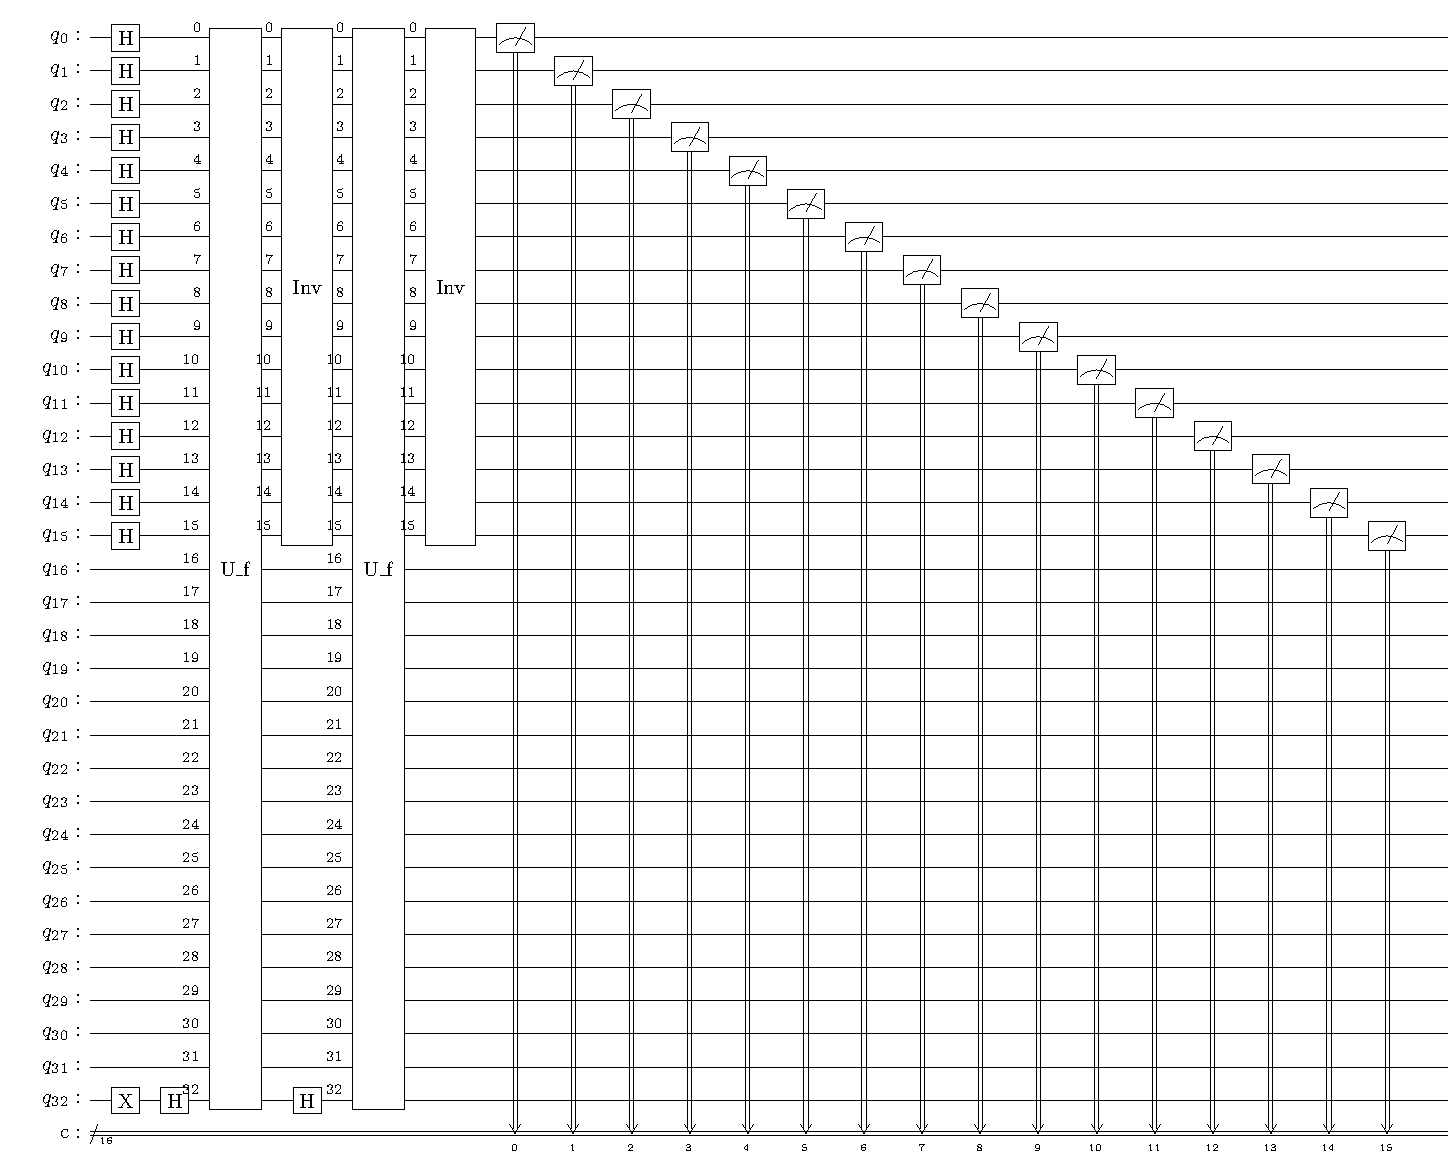
\includegraphics[width=0.9\linewidth]{saes21/grover-2-iter.pdf}
    \caption{Grover's Attack (2 iterations)}
    \label{fig:grov21}
\end{figure}



\begin{figure}[h!]
    \centering
    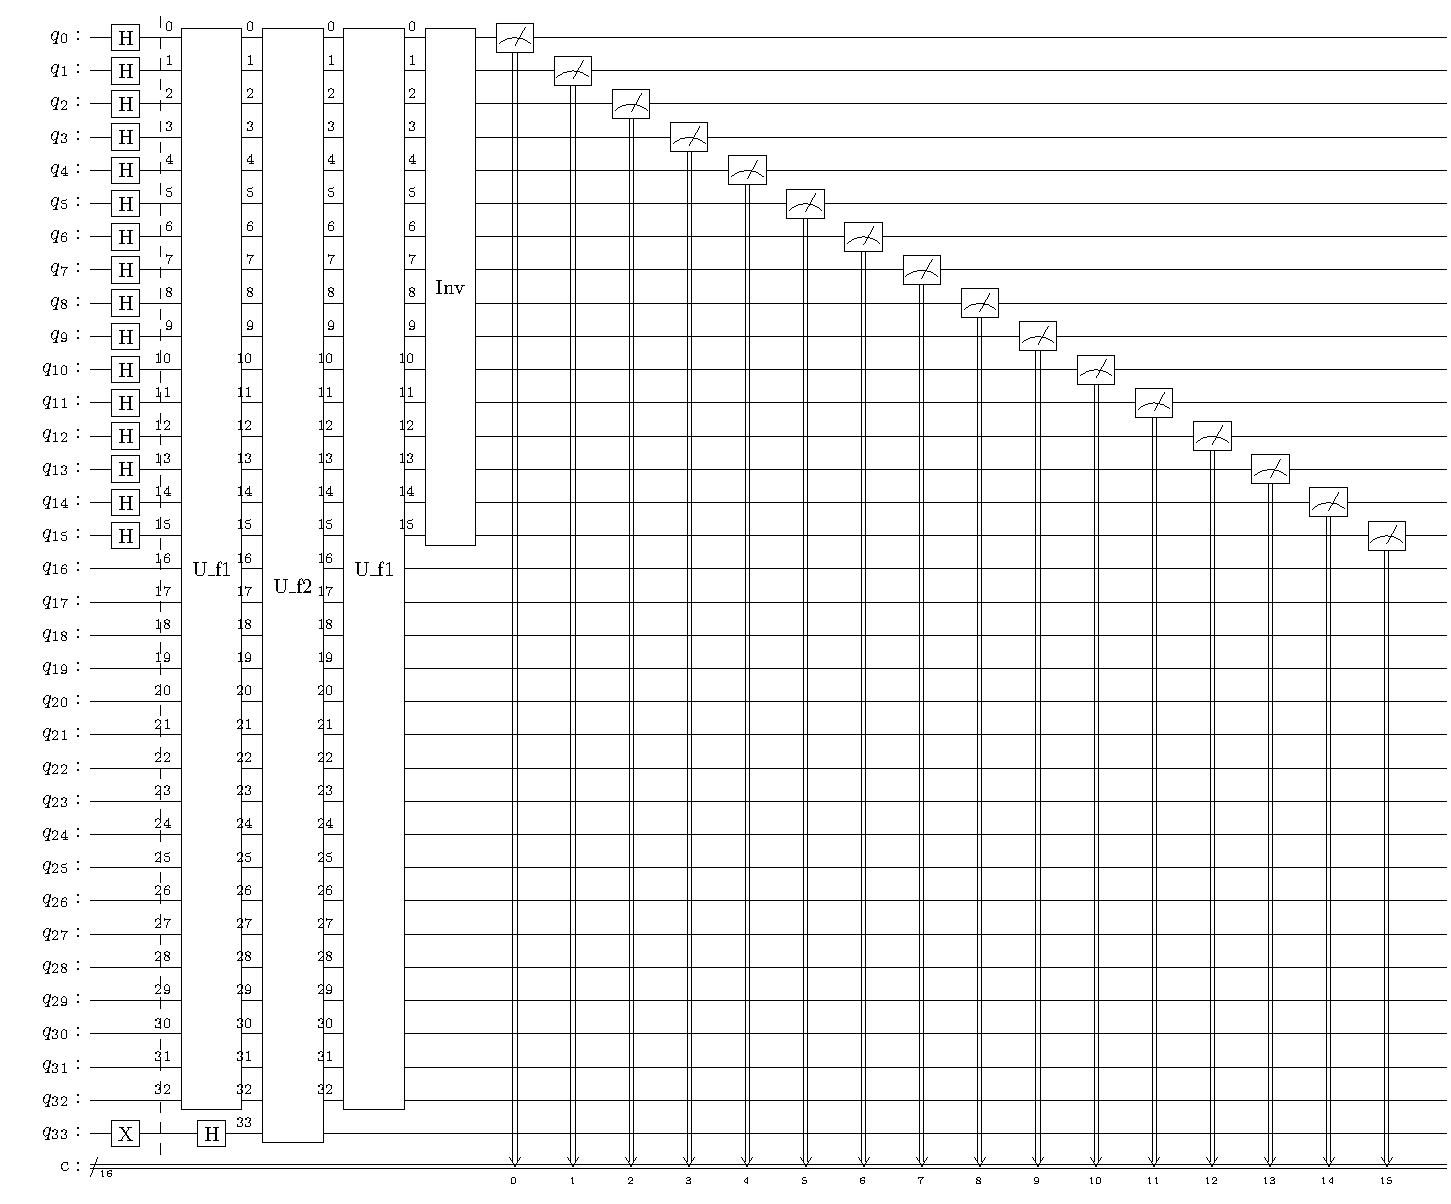
\includegraphics[width=0.9\linewidth]{saes21/grover-coupling-1-iter.pdf}
    \caption{Grover's Attack for unique key with r = 2 (1 iteration)}
    \label{fig:grov21u}
\end{figure}



\begin{center}
\begin{table}[h!]
    \centering
    \begin{tabular}{ |c|c|c|c|c|c|c| } 
     \hline
       & Qubits & X & CX & CCX & Ancilla \\ \hline
     Key expansion & 32 & 10& 568 & 192 & 8 \\ \hline
     Encryption & 32 & 16 & 512 & 384 & - \\ \hline
     Total & 64 & 26 & 1080 & 576 & 8 \\ \hline
     Key expansion & 16 & 19& 56 & 48 & - \\ \hline
     Encryption & 16 & 16 & 88 & 48 & - \\ \hline
     Total & 32 & 35 & 144 & 96 & - \\ \hline
     My Code & 32 & 35 & 144 & 96 & - \\ \hline
    \end{tabular}
    \caption{Comparison of cost for QSAES18\cite{Almazrooie} and QSAES21\cite{Jang} }
    \label{tab:cost21}
\end{table}
\end{center}

The cost was heavily reduced due to optimizations in Sbox, key expansion, and mix columns circuit. The cost of a Grover's Attack can be calculated as follows. Since the encryption is performed twice (two plaintext-ciphertext pairs) and also the reversible circuit is added, the total cost of Grover's Attack to find a unique key is

\begin{equation*}
    2\times 2\times \frac{\pi}{4}\sqrt{2^{16}}
\end{equation*}

\section{SIMON}\label{sec:simon}
\cite{gos} discusses Grover's Attack on lightweight block cipher SIMON 2n/mn using $O(mn + 2nr)$ qubits where $r$ is the count of chosen plaintext-ciphertext pairs. We briefly describe the SIMON cipher and then its quantum circuit. Figure \ref{fig:ors} shows one round of the SIMON cipher. SIMON has 10 different block sizes shown in Table \ref{tab:sp}. In SIMON 2n/mn, 2n refers to the block size and mn refers to the key size. 

The equation below describes one round of the SIMON cipher.
\begin{equation}\label{eq:simonfun}
    F(x,y) = (y\oplus (S^1(x)\wedge S^8(x)) \oplus S^2(x) \oplus k, x)
\end{equation}

$S^j(x)$ denotes left circular shift by j bits. $PT_1, PT_2$ are also referred as $L_i, R_i$ and $CT_1, CT_2$ are also referred as $L_{i+1}, R_{i+1}$. $L_i, R_i$ are $n$ bit strings as input to the $i^{th}$ round and $k$ is the round key.

The key expansion has 3 different methods which depend on the key size. For the first $m$ rounds, the round keys are initialized from the master key. For the remaining T-m rounds, the round keys are generated using the function given below:

\begin{equation}
 k_{m+i} = 
 \begin{cases} 
      c_i \oplus k_i \oplus S^{-3}(k_{i+1}) \oplus S^{-4}(k_{i+1}) &  m = 2 \\
      c_i \oplus k_i \oplus S^{-3}(k_{i+2}) \oplus S^{-4}(k_{i+2}) &  m = 3 \\
      c_i \oplus k_i \oplus S^{-1}(k_{i+1}) \oplus S^{-3}(k_{i+3}) \oplus S^{-4}(k_{i+3}) &  m = 4
  \end{cases}
\end{equation}

$c_i$ denotes the round constants.

\begin{figure}[h!]
    \centering
    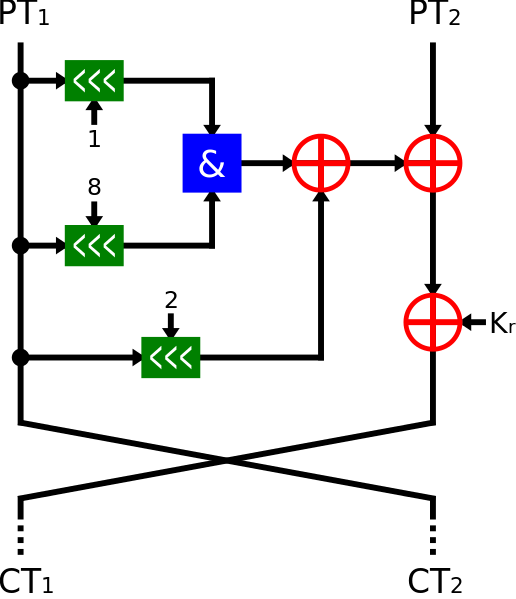
\includegraphics[width=0.5\linewidth]{simon/simon.png}
    \caption{One round of SIMON \cite{wiki:simon}}
    \label{fig:ors}
\end{figure}

\begin{center}
\begin{table}[h!]
    \centering
    \begin{tabular}{ |c|c|c|c|c| } 
     \hline
     Word size (n) & Block size (2n)  & keywords (m) & Key size (mn) & Rounds (T) \\ \hline
     16 & 32 & 4 & 64 & 32  \\ \hline 
     24 & 48 & 3,4 & 72,96 & 36,36 \\ \hline
     32 & 64 & 3,4 & 96,128 & 42,44 \\ \hline
     48 & 96 & 2,3 & 96,144 & 52,54  \\ \hline
     64 & 128 & 2,3,4 & 128,192,256 & 68,69,72  \\ \hline
     
    \end{tabular}
    \caption{Parameters of SIMON cipher \cite{gos}}
    \label{tab:sp}
\end{table}
\end{center}



\section{Quantum SIMON}\label{sec:qsimon}
We now describe the design of the quantum circuit for SIMON as proposed by \cite{gos} and call it QSIMON. Let the initial state be $L_0, R_0$. From equation \ref{eq:simonfun}, we can construct the path for $i^{th}$ bit from $R_0$ which can be written as

\begin{equation*}
    R_2(i) = L_1(i) = R_0(i) \oplus (L_0(i+1)mod(n) \wedge L_0(i+8)mod(n)) \oplus L_0(i+2)mod(n) \oplus k_0
\end{equation*}
In quantum circuit, after initializing $L_0, R_0$, we can use the qubits of $R_0$ for storing $L_1$ and $L_0$ becomes $R_1$. This process can be continued for further rounds. This eliminates the need for ancilla qubits. 

For computing $R_2(i)$, we can use the following operations:
\begin{enumerate}
    \item CCX($L_0(i+1)mod(n), L_0(i+8)mod(n), R_0(i)$)
    \item CX($L_0(i+2)mod(n), R_0(i)$)
    \item CX($k_0(i), R_0(i)$)
\end{enumerate}

The same process can be followed for $L_2$ and then for other rounds. Calculating the number of gates for one round of SIMON, we can see that we need $n$ Toffoli gates and $2n$ CNOT gates for a single round. For $j$ rounds, we need $jn$ and $2jn$ Toffoli and CNOT gates respectively.

We define three functions that together form one round of the QSIMON as shown in Figure \ref{fig:sqs}. Using these three functions we can create QSIMON. 2 round construction of QSMION is shown in Figure \ref{fig:2rqs}.

\begin{figure}[h!]
\minipage{0.32\textwidth}
   
   \resizebox{4cm}{!}{
   \begin{quantikz}
    \lstick{$\ket{b}$} &[2mm] \ctrl{1} & \qw & \rstick{$\ket{b}$} \qw  \\
    \lstick{$\ket{a}$} &[2mm] \gate{F} & \qw & \rstick{$\ket{a\oplus S^1(b)S^8(b)}$} \qw \\
    \end{quantikz}
    }
\endminipage\hfill
\minipage{0.32\textwidth}
  \resizebox{4cm}{!}{
   \begin{quantikz}
    \lstick{$\ket{b}$} &[2mm] \ctrl{1} & \qw & \rstick{$\ket{b}$} \qw  \\
    \lstick{$\ket{a}$} &[2mm] \gate{G} & \qw & \rstick{$\ket{a\oplus S^2(b)}$} \qw \\
    \end{quantikz}
    }
\endminipage\hfill
\minipage{0.32\textwidth}%
 \resizebox{4cm}{!}{
   \begin{quantikz}
    \lstick{$\ket{b}$} &[2mm] \ctrl{1} & \qw & \rstick{$\ket{b}$} \qw  \\
    \lstick{$\ket{a}$} &[2mm] \gate{H} & \qw & \rstick{$\ket{a\oplus b}$} \qw \\
    \end{quantikz}
    }
\endminipage
\caption{Subroutines for one round of QSIMON}
\label{fig:sqs}
\end{figure}

\begin{figure}[h!]
    \centering
    \begin{quantikz}
    \lstick{$\ket{k_0}$} &[2mm] \qw & \qw & \ctrl{2} & \rstick{$\ket{k_1}$} \qw  & & &\qw &\qw & \ctrl{1} &\qw & \rstick{$\ket{k_2}$} \qw \\
    \lstick{$\ket{L_0}$} &[2mm] \ctrl{1} & \ctrl{1} & \qw & \rstick{$\ket{R_1}$} \qw & & & \gate{F} & \gate{G} &\gate{H} &\qw & \rstick{$\ket{L_2}$} \qw  \\
    \lstick{$\ket{R_0}$} &[2mm] \gate{F} & \gate{G} & \gate{H} & \qw \rstick{$\ket{L_1}$} & & & \ctrl{-1} & \ctrl{-1} &\qw &\qw & \rstick{$\ket{R_2}$} \qw   \\
    \end{quantikz}
    \caption{2 Round of QSIMON}
    \label{fig:2rqs}
\end{figure}

\subsection{Key Expansion}

Define a function as 
\begin{equation*}
    R_q(a,b) = (S^{-i}(b)\oplus a, b)
\end{equation*}
This function will be used in the circuit of key expansion. The quantum circuit for this equation is shown in Figure \ref{fig:keeqs}

\begin{figure}[h!]
    \centering
    \begin{quantikz}
    \lstick{$\ket{b}$} &[2mm] \ctrl{1} & \qw & \rstick{$\ket{b}$} \qw  \\
    \lstick{$\ket{a}$} &[2mm] \gate{R_q} & \qw & \rstick{$\ket{(S^{-i}(b)\oplus a}$} \qw \\
    \end{quantikz}
    \caption{Quantum circuit for $R_q(a,b)$}
    \label{fig:keeqs}
\end{figure}

Consider the case for $m=2$. The key size is $2n$, so we have two keywords $k_0, k_1$ which are used in the first 2 rounds. For the rest of the rounds, round keys are derived from $k_0, k_1$. The third round key can be calculated using the following steps:

\begin{enumerate}
    \item CX($k_1(i-3) mod(n) , k_0(i)$)
    \item CX($k_1(i-4) mod(n), k_0(i)$)
    \item NOT($k_0(i)$) if $i^{th}$ bit of round constant is true
\end{enumerate}

The above steps are illustrated in Figure \ref{fig:kem2}

\begin{figure}[h!]
    \centering
    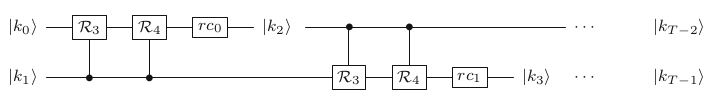
\includegraphics[width=\linewidth]{simon/m2.png}
    \caption{Key expansion for m = 2 \cite{gos}}
    \label{fig:kem2}
\end{figure}

We can follow a similar procedure for $m= 3$ and $4$. The quantum circuits for them is shown in Figure \ref{fig:kem3} and \ref{fig:kem4} respectively.


\begin{figure}[h!]
    \centering
    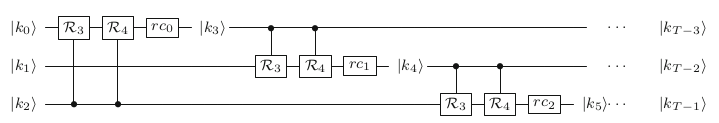
\includegraphics[width=\linewidth]{simon/m3.png}
    \caption{Key expansion for m = 3 \cite{gos}}
    \label{fig:kem3}
\end{figure}


\begin{figure}[h!]
    \centering
    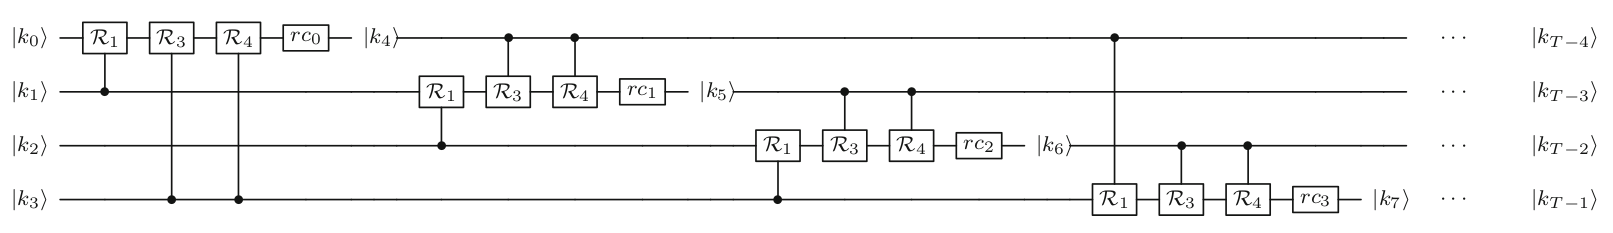
\includegraphics[width=\linewidth]{simon/m4.png}
    \caption{Key expansion for m = 4 \cite{gos}}
    \label{fig:kem4}
\end{figure}

QSIMON for $m=2$ is shown in Figure \ref{fig:qsim2}

\begin{figure}[h!]
    \centering
    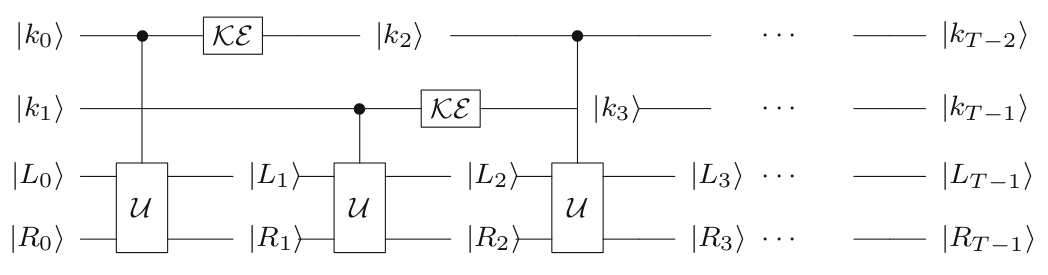
\includegraphics[width=\linewidth]{simon/qsim2.png}
    \caption{QSIMON for m = 2 \cite{gos}}
    \label{fig:qsim2}
\end{figure}

For 1 round we need 2n, 2n, and 3n CNOT gates for m = 2,3 and 4 respectively and $n'$ NOT gates which depend on the count of true bits in round constant. For remaining T-m rounds, the key expansion procedure requires 2n(T-m), 2n(T-m), and 3n(T-m) CNOT gates for m = 2,3, and 4 respectively and n'(T-m) NOT gates.
 
\subsection{Grover's Attack}\label{sec:qsimgrov}

\begin{figure}[h!]
    \centering
    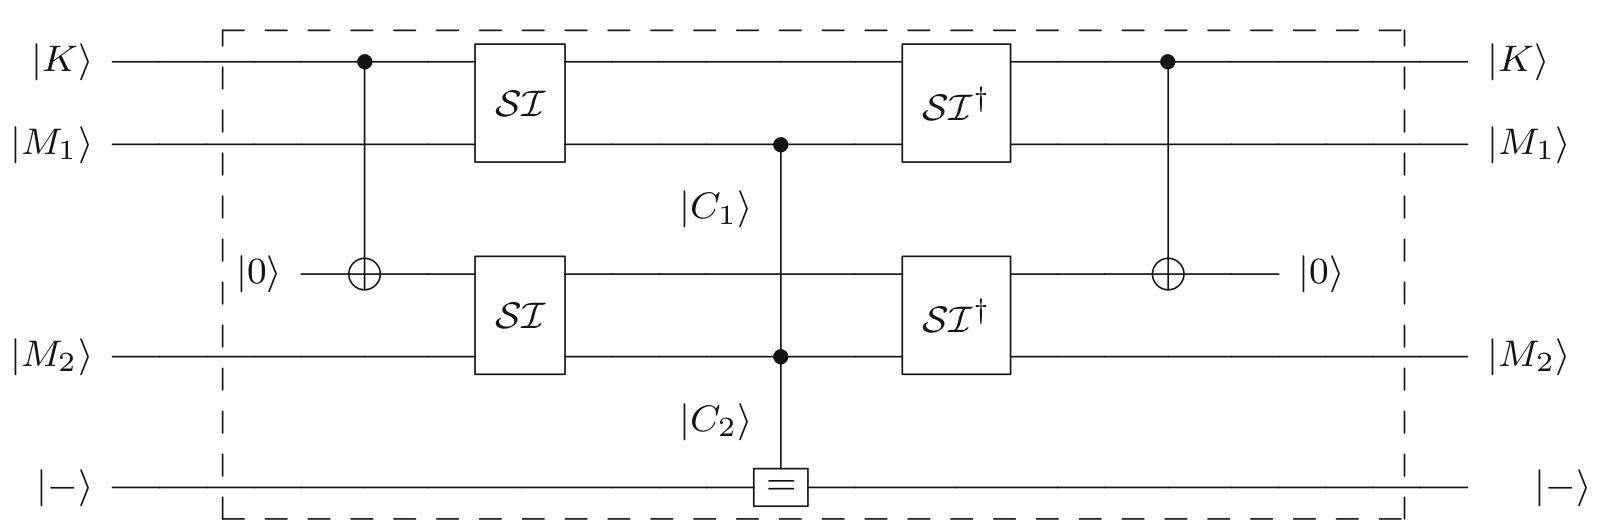
\includegraphics[width=\linewidth]{simon/qsimgrov.png}
    \caption{Grover's Attack on QSIMON \cite{gos}}
    \label{fig:qsimgrov}
\end{figure}

We will discuss the implementation of Grover's Oracle for a successful Grover's Attack to obtain the unique key. If we have $r$ chosen plaintext-ciphertext pairs then the Grover's Oracle circuit can be implemented using $r$ QSIMON oracles in parallel along with $r$ QSIMON$\dagger$ oracles (reversibility). This implementation is shown in Figure \ref{fig:qsimgrov}


The authors were able to successfully recover the key for a round reduced version of SIMON. For finding a unique key we need precisely 2 plaintext-ciphertext pairs i.e. r = 2. Grover's Oracle compares $2n$ qubits ($n$ qubits of $C_1$ and $n$ qubits of $C_2$) using unbounded Toffoli gate \cite{mcmt}. This is when r = 2. In general, we require $2nr$ CNOT gates. $mn$ qubits are needed for the master key. Therefore the total qubits complexity is of the order $O(mn + 2nr)$. The authors have provided tables that shows cost of each variant of SIMON \cite{gos}.

\section{PRESENT}\label{sec:present}

PRESENT\cite{present} is an Ultra-lightweight block cipher and has a substitution permutation network. It has a block length of 64 bits and supports 80 and 128-bit key sizes. Figure \ref{fig:spp} shows SP network for PRESENT cipher.

\begin{figure}[h!]
    \centering
    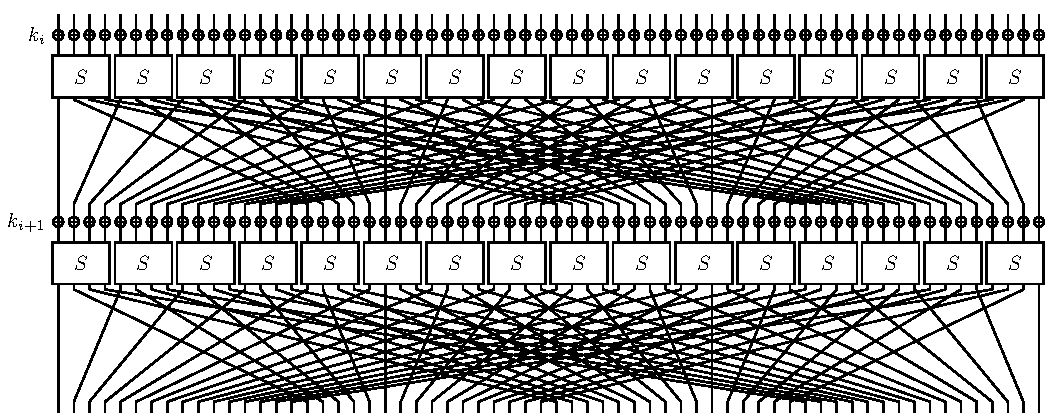
\includegraphics[width=\linewidth]{present/PRESENT_diagram.pdf}
    \caption{SP network for PRESENT cipher \cite{presentdiagram}}
    \label{fig:spp}
\end{figure}

\subsection{Cipher Design}
With 31 rounds, the Present-80 is an example of an SP network. A xor of the round key is followed by a 4-bit non-linear substitution layer and linear bit-wise permutation in each round. During each round, the 4-bit SBox is applied 16 times in parallel to the 64-bit input. The higher level pseudo-code for implementing the encryption algorithm is shown in Figure \ref{fig:pseudocode}. A top-level description of the encryption algorithm can be found in Figure \ref{fig:top-level-diagram}.

\tikzset{
    block/.style = {
        draw, 
        fill=white, 
        rectangle, 
        minimum height=1.8em, 
        minimum width = 10em
    },
    block2/.style = {
        draw, 
        fill=white, 
        rectangle, 
        minimum height=3.7em, 
        minimum width=6em
    },
    sum/.style = {
        draw, 
        fill=white, 
        circle, 
        inner sep=0pt,
        minimum size = 0.5cm
    },
    pinstyle/.style = {
        pin edge={to-,thin,black}
    }
}

\begin{figure}[h!]
    \captionof{figure}{A top-level algorithmic description of present}\label{fig:top-level}
    \centering
    \begin{subfigure}[b]{0.3\linewidth}
        \begin{algorithmic}
            \STATE{generateRoundKeys()}
            \FOR{$i=1$ \TO $31$ }
                \STATE {addRoundKey(\textsc{State},$K_i$)} 
                \STATE {sBoxLayer(\textsc{State})} 
                \STATE {pLayer(\textsc{State})} 
            \ENDFOR
            \STATE addRoundKey(\textsc{State},$K_{32}$)
        \end{algorithmic}
        \caption{}
        \label{fig:pseudocode}
    \end{subfigure}
    \hspace{60pt}
    \begin{subfigure}[b]{0.5\linewidth}
        \begin{tikzpicture}[auto, node distance=2cm,>=latex',scale=0.6, every node/.style={scale=0.6}]
            % nodes
            \node [sum] (sum1) {+};
            \node [block,above of=sum1,node distance=1cm] (plaintext) {plaintext};
            \node [block,right of=plaintext,node distance=5cm] (keyregister) {key register};
            \node [block,below of=sum1,node distance=1cm] (sBoxLayer) {sBoxLayer};
            \node [block,below of=sBoxLayer,node distance=0.7cm] (pLayer) {pLayer};
            \node [block,below of=pLayer,node distance=4cm] (sBoxLayer2) {sBoxLayer};
            \node [block,below of=sBoxLayer2,node distance=0.7cm] (pLayer2) {pLayer};
            \node [sum, below of=pLayer2,node distance=1cm] (sum2) {+};
            \node [block,below of=sum2,node distance=1cm] (ciphertext) {ciphertext};
            
            \node [block2,below of=keyregister,node distance=2.35cm] (update) {update};
            \node [block2,below of=update,node distance=4.7cm] (update2) {update};
        
            % arrows
            \draw [->] (plaintext) -- (sum1);
            \draw [->] (sum1) -- (sBoxLayer);
            \draw [->] (pLayer2) -- (sum2);
            \draw [->] (sum2) -- (ciphertext);
            \draw [->] (keyregister) -- (update);
            \draw [->,dashed] (update) -- (update2);
            \draw [->,dashed] (pLayer) -- (sBoxLayer2);
            \draw [->] (keyregister)  |- node[above left= 0pt] {addRoundKey            }    (sum1);
            \draw [->] (update2) |- node[above left= 0pt]{addRoundKey            }   (sum2);
        \end{tikzpicture}
        \caption{} 
        \label{fig:top-level-diagram}
    \end{subfigure}
  
  \end{figure}

\subsubsection{Add Round Key}
Provided the round key $K_i = k_{63},k_{62} \dots k_0$ for $1\leq i \leq 32$ and the current state $S = s_{63},s_{62}\dots s_0$, addRoundKey performs the following operation
\begin{eqnarray*}
    S \xrightarrow{} S \oplus K_i \\
    \implies s_t \xrightarrow[]{} s_t \oplus k_t 
\end{eqnarray*}
for $0\leq t\leq 63$.

\subsubsection{Substitution Layer}
The substitution box is 4-bit to 4-bit mapping. Table \ref{tab:pSbox} shows the mapping of Sbox in Hexadecimal notation. The 4-bit S-Box is independently repeated 16 times to cover the 64-bit block.
\begin{figure}[h!]
    \centering
    \begin{tabular}{ |c||c|c|c|c|c|c|c|c|c|c|c|c|c|c|c|c| }
        \hline
        $x$ & 0 & 1 & 2 & 3&4& 5& 6&7&8&9&A&B&C&D&E&F  \\ \hline
        $S[x]$& C & 5 & 6& B &9 &0 &A &D& 3& E &F& 8& 4 &7& 1& 2 \\ \hline
    \end{tabular}
    \captionof{table}{Present Sbox}
    \label{tab:pSbox}
\end{figure}
The substitution box is a mapping $S:\mathbb{F}_2^4\xrightarrow[]{}\mathbb{F}_2^4$ where $\mathbb{F}$ is a finite field. 
\subsubsection{Permutation Layer} 
The permutation layer is a bit permutation. The permutation function P(i) maps the $i^{th}$ bit of input to P(i) in the output of the permutation layer. The Table {\ref{tab:pLayer}} is the mapping of P(i) in tabular form. 
\begin{figure}[h!]
    \centering
    \begin{tabular}{ |c||c|c|c|c|c|c|c|c|c|c|c|c|c|c|c|c| }
        \hline
        i& 0 &1 &2 &3& 4& 5& 6 &7 &8 &9 &10 &11 &12 &13 &14 &15 \\
        P(i) &0& 16& 32& 48& 1& 17& 33&49& 2 &18& 34& 50& 3 &19 &35 &51 \\\hline\hline
        i &16& 17& 18& 19& 20& 21 &22& 23 &24 &25 &26 &27 &28 &29 &30 &31 \\
        P(i)& 4 &20 &36& 52& 5& 21 &37& 53& 6 &22& 38& 54& 7 &23 &39 &55 \\\hline\hline
        i &32& 33& 34& 35& 36& 37 &38& 39 &40 &41 &42 &43 &44 &45 &46 &47 \\
        P(i) &8 &24& 40& 56 &9& 25 &41 &57 &10 &26 &42 &58 &11 &27 &43 &59 \\\hline\hline
        i &48& 49& 50 &51 &52 &53& 54& 55 &56 &57 &58 &59 &60 &61 &62 &63 \\
        P(i) &12& 28& 44&60& 13 &29& 45& 61 &14 &30 &46 &62 &15 &31 &47 &63 \\\hline
    \end{tabular}
    \captionof{table}{Present pLayer}
    \label{tab:pLayer}
\end{figure}
\subsubsection{Key schedule Algorithm}\label{sec:qpksa}
The Present cipher supports 80-bit or 128-bit long key, in this section we discuss the 80-bit key schedule algorithm. Firstly, the initial 80-bit key is stored in a key register $K$ and is represented as $K = k_{79}k_{78}$..$k_0$. At any round $i$, PRESENT extracts the 64-bits round key $K_i = \mathrm{k_{63}}\mathrm{k_{62}}$..$\mathrm{k_{0s}}$ from the current Key (left most 64 bits) register as follows : 
\begin{equation*}
    K_i = \mathrm{k_{63}}\mathrm{k_{62}}..\mathrm{k_{0s}} = k_{79}k_{78}..k_{16}
\end{equation*}
After round key extraction, the key register $K$ is updated according to the following rules : 
\begin{enumerate}
    \item The contents of the key register $K$ is rotated by 61-bits to the left.
    \begin{equation*}
        [k_{79}k_{78}..k_{0}] = [k_{18}k_{17}..k_{20}k_{19}]
    \end{equation*}
    \item The 4-leftmost bits of the key register $K$ is passed through the PRESENT S-box.
    \begin{equation*}
        [k_{79}k_{78}k_{77}k_{76}] = S[k_{79}k_{78}k_{77}k_{76}]
    \end{equation*}
    \item The 5-bits of key register $k$, $k_{19}k_{18}k_{17}k_{16}k_{15}$ is exclusive-ored with the least significant bits of the round counter value $i$. 
    \begin{equation*}
        [k_{19}k_{18}k_{17}k_{16}k_{15}] = [k_{19}k_{18}k_{17}k_{16}k_{15}] \oplus round-counter
    \end{equation*}
\end{enumerate}

\section{QPRESENT}\label{sec:qpresent}
We now describe the design of the quantum circuit for SIMON as proposed by \cite{gop} and call it QPRESENT. QPRESENT only allocates qubits for plaintext and key and does not allocate ancilla qubits. 

\subsection{Add Round Key}
Add round key can be implemented simply using 64 CNOT gates from key to plaintext.

\subsection{Sbox}
Instead of implementing the algebraic normal form of PRESENT Sbox, authors of \cite{gop} used LIGHTER-R tool \cite{LighterR} for optimized implementation of Sbox with no ancilla qubits and optimal circuit depth. The quantum circuit for Sbox is shown in Figure \ref{fig:qpsbox}

\begin{figure}[h!]
    \centering
    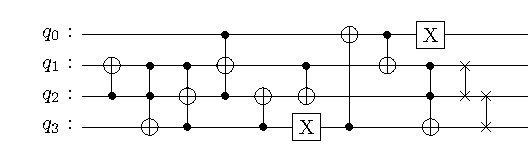
\includegraphics[width=\linewidth]{present/sbox.pdf}
    \caption{Sbox for QPRESENT}
    \label{fig:qpsbox}
\end{figure}

The qubits at the output are permuted and therefore two SWAP gates are added at the end of the circuit.

\subsection{Permutation Layer}
The permutation layer as shown in Table \ref{tab:pLayer} can be implemented using only SWAP gates. Bits 0,21,42 and 63 do not change their positions. Other 60 bits can be grouped in 3-bit groups of 20 bits each. Each 3-bit group is a permutation. For example, 1 map to 16, 16 maps to 4, and then 4 maps to 1. This can be implemented as follows 

\begin{equation*}
    \begin{aligned}
        SWAP(x_1, x_4) \\
        SWAP(x_4,x_{16})
    \end{aligned}
\end{equation*}

The same is followed for the remaining bits. Since we do not count SWAP gates in quantum resources as this operation can be achieved by rewiring, the quantum cost for the permutation layer of QPRESENT is zero.

\subsection{Key schedule Algorithm}
As described in Section \ref{sec:qpksa}, to implement the key schedule algorithm in the quantum circuit we use algorithm \ref{proc:keqp}. The input is an 80-bit key and the output is a 64-bit round key.

\begin{codebox}
\Procname{$\proc{Key Expansion for QPRESENT}(K = k_{79}k_{78}$..$k_0)$}\label{proc:keqp}
\li $k = \mathrm{k_{63}}\mathrm{k_{62}}..\mathrm{k_{0s}} = k_{79}k_{78}..k_{16}$
\li $k \gets k \gg 19$
\li $[k_{79}k_{78}k_{77}k_{76}] = S[k_{79}k_{78}k_{77}k_{76}]$
\li $[k_{19}k_{18}k_{17}k_{16}k_{15}] = X[k_{19}k_{18}k_{17}k_{16}k_{15}]$
\li \Return $k$
\end{codebox}

The operations will be performed on left-most 64 bits denoted by variable $k$ on line 1. Instead of rotating 61 bits to left, rotate 19 bits to right using SWAP gates. The leftmost 4 bits are passed through Sbox and then the round constant is XORed with bits $k_{19}k_{18}k_{17}k_{16}k_{15}$ using NOT gate.


\subsection{Grover's Attack}
Similar to Grover's Attack on SIMON as described in Section \ref{sec:qsimgrov}, the quantum circuit for Grover's Attack can be used. Figure \ref{fig:qpgrov} shows the circuit.

\begin{figure}[h!]
    \centering
    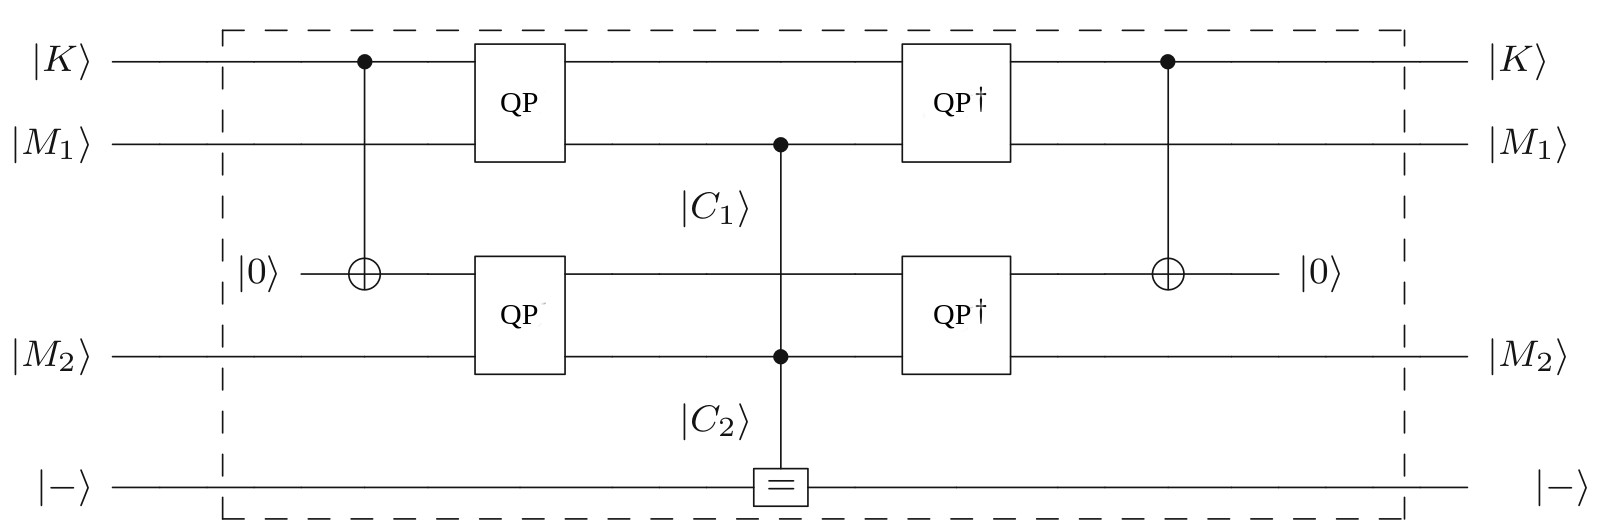
\includegraphics[width=\linewidth]{present/qpgrov.jpg}
    \caption{Grover's Attack on QPRESENT for r = 2}
    \label{fig:qpgrov}
\end{figure}

We compare the cost of Quantum resources of QPRESENT 64/80 and QSIMON 64/128 shown in Table \ref{tab:cqpqs}.

\begin{center}
\begin{table}[h!]
    \centering
    \begin{tabular}{ |c|c|c|c|c|c|c|c| } 
     \hline
     Cipher  & Qubits & X & CX & CCX & Ancilla & Depth \\ \hline
     QPRESENT 64/80 & 144 & 1118 & 4683 & 2108 & - & 311 \\ \hline
     QSIMON 64/128 & 192 &1216 & 7396 & 1408 & - & 2643\\ \hline
    \end{tabular}
    \caption{Comparison of cost for QPRESENT 64/80 \cite{gop} and QSIMON 64/128\cite{gos} }
    \label{tab:cqpqs}
\end{table}
\end{center}

Since the key sizes and number of rounds of both the ciphers are different, the comparison is not fruitful. There is no Sbox in the case of SIMON which can lower its cost complexity as Sbox's quantum circuit is a bottleneck in circuit's depth but also the cost of permutation layer in case of PRESENT is zero due to the use of only SWAP gates.

\section{Grover on AES}\label{sec:grovaes}

This section describes the work of \cite{aeslowmc} in brief for AES-128. They have studied quantum circuits under the MAXDEPTH constraint.


Let $N=2^k$ be the key search space and let $M \geq 1$ is the number of solutions that exists in $N$. We know that $sin^2(\theta) = \frac{M}{N}$ for $0 < \theta \leq \frac{\pi}{2}$ and for $M \ll N$ we have $\theta \approx \sqrt{\frac{M}{N}}$. The probability of finding one of the $M$ solutions after $t$ iterations is defined as 
\begin{equation*}
    p(t) = sin^2((2t+1)\theta)
\end{equation*}
which after solving for 1 gives $t\approx \frac{\pi}{4\theta} = \frac{\pi}{4} \sqrt{\frac{M}{N}}$.

\subsection{Key search}

Let $E_K(m) = c$ denote the encryption of message $m \in \{ 0,1\}^n$ by key $K\in \{0,1\}^k$ to ciphertext $c$. For $r$ plaintext-ciphertext pairs we have $E_K(m_i) = c_i$. Then the Grover's Oracle is defined as:

\begin{equation*}
 f(K) = 
 \begin{cases} 
      1 & E_K(m_i) = c_i  \\
      0 & else 
  \end{cases}
\end{equation*}

It is possible that multiple keys other than $K$ lead to the same ciphertext from the given plaintext. The authors call them spurious keys.

The problem is to find the optimal number $r$ such that the probability of finding a spurious key is minimal. Assume $K$ is the actual key we're interested in and $K'$ is spurious. Then the probability that given $K \not = K'$, $E_K(m) = E_{K'}(m)$ is given as:
\begin{equation*}
    P_{K \not = K'}(E_K(m) = E_{K'}(m)) = \frac{1}{2^n}
\end{equation*}

for $r$ plaintext-ciphertext pairs, we have:
\begin{equation*}
    p = P_{K \not = K'}((E_K(m_1), E_K(m_2), \dots ,E_K(m_r) ) = (E_{K'}(m_1),E_{K'}(m_2), \dots, E_{K'}(m_r)) )) = \left(\frac{1}{2^n}\right)^r = 2^{-nr}
\end{equation*}

Let $Y$ be a random variable that describes the count of spurious keys for given key $K$ and $r$ plaintext-ciphertext pairs. $Y$ is then distributed binomially:
\begin{equation*}
    P(Y = y) = {2^k - 1 \choose y} p^y(1-p)^{2^k - 1- y}
\end{equation*}

We can approximate this to poission distribution with $\lambda = (2^k-1)p = (2^k - 1)2^{-rn} $
\begin{equation*}
    P(Y=y) = \frac{e^{-\lambda}\lambda^k}{y!} \approx  \frac{e^{-2^{k-rn}}2^{(k-rn)y}}{y!}
\end{equation*}

The probability that no spurious key exists i.e. $P(Y = 0) \approx e^{-2^{k-rn}}$. We need to maximise this probability which will happen when $rn > k$ or we can choose $r = \left\lceil \frac{k}{n} \right\rceil$.

\subsection{Parallelization of Grover}

Two ways have been described in \cite{tsc} for parallelizing Grover's algorithm denoted by inner and outer parallelization. In outer parallelization, multiple instances of the full Grover's algorithm are run on different machines simultaneously for a reduced number of iterations. The outputs can then be checked classically. In the case of inner parallelization, the search space is divided into multiple disjoint subsets and each machine is assigned one subset. Since each machine has a smaller search space, this reduces the number of iterations on each machine.

\cite{zalka} found that there is a gain of $\sqrt{S}$ in the number of iterations for $S$ parallel machines. This is inefficient as we gain only $\sqrt{S}$ factor in the depth of the quantum circuit whereas the width has become $S$ times the original. \cite{aeslowmc} uses inner parallelization.

\subsubsection{Why inner parallelization?}

If we use outer parallelization, then the probability that we find the correct key after $t$ iterations is $p_S(t) = 1 - (1-p(t))^S$. In each machine the number of iterations will be $t_S = \frac{\pi}{4\theta\sqrt{S}}$. Table \ref{tab:pval} highlights some of the probabilities for different values of $S$.


\begin{center}
\begin{table}[h!]
    \centering
    \begin{tabular}{ |c|c| } 
     \hline
     S & $p_S(t)$ \\ \hline
     1 & $\approx 1$ \\ \hline
     2 & 0.96 \\ \hline
     3 & 0.94 \\ \hline
    \end{tabular}
    \caption{Probabilities of finding the correct key for different count of parallel machines }
    \label{tab:pval}
\end{table}
\end{center}

We can find a general expression by using the series expansion of $sin(x)$ for larger values of $S$.

\begin{equation*}
    p_S(t_S) = 1 - \left( 1 - \frac{\pi^2}{4S} + O\left(\frac{1}{S^2}\right) \right)^S 
\end{equation*}

As $S$ tends to $\infty$, the above value approaches to $1 - e^{\frac{-\pi^2}{4}} \approx 0.91$. This implies by just by increasing the number of parallel machines $S$, one cannot get a probability near 1 for finding the correct key. For the case of inner parallelization, the correct key exists in one of the subsets only, and with $t_S$ iterations, the machine has a near 1 probability of finding it and other machines will not find it. Therefore inner parallelization has a higher chance of obtaining the correct key as compared to outer parallelization.

One thing to note is spurious keys. If spurious keys are present in a subset with the correct key not in that subset, then the spurious key can be discarded classically after the experiment. The probability that spurious keys fall into the subset with the correct key is given by:
\begin{equation*}
    \sum_{y = 1}^\infty P(Y = y) = 1 - e^{-\frac{2^{k-rn}}{S}} 
\end{equation*}
In the above equation, we have replaced $2^k$ by $2^k/S$ which is the subset size. In essence, increasing $S$ makes the above probability small. 
\subsection{Quantum Circuit Design}

The authors use AND gate (Figure \ref{fig:and}) instead of Toffoli gate(Figure \ref{fig:toff}). The decomposition of the Toffoli gate is to 7 T gates, 8 Clifford gates with a T-depth(number of T gates in a row\cite{stack}) 4 and total depth 11 whereas AND gate used 4 T gates, 11 Clifford gates with T-depth 1 and total depth 8. AND gate uses one ancilla qubit which is released after the operation.


\begin{figure}[h!]
    \centering
    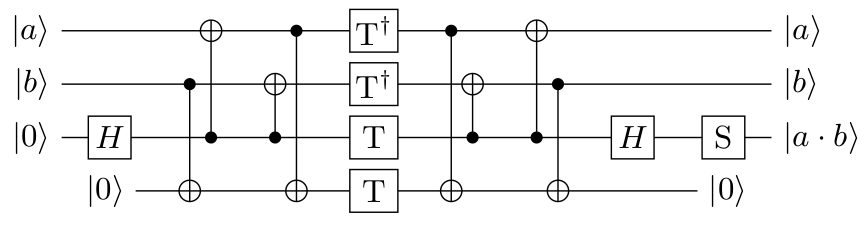
\includegraphics[width=\linewidth]{aes/and.png}
    \caption{AND Gate \cite{aeslowmc}}
    \label{fig:and}
\end{figure}

\begin{figure}[h!]
    \centering
    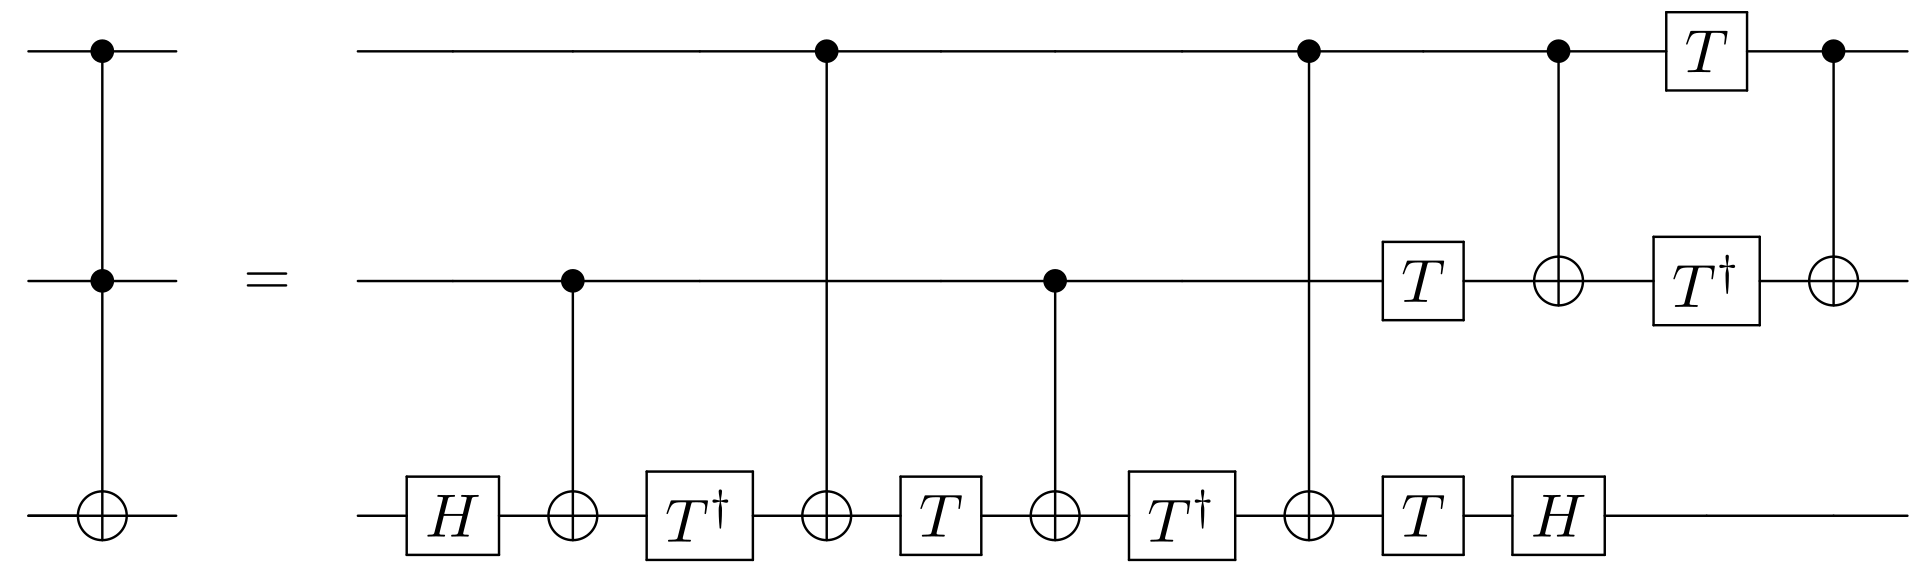
\includegraphics[width=\linewidth]{aes/toffoli.png}
    \caption{Toffoli gate decomposition\cite{wiki:toff}}
    \label{fig:toff}
\end{figure}

\subsubsection{Quantum circuit for linear maps}
Linear mapping $f:\mathbb{F}_2^n \rightarrow \mathbb{F}_2^m$ are building blocks of AES. If a linear map is invertible then it can be computed in place using PLU decomposition, where L and U are lower and upper triangular matrices implemented using CNOT gates and P is a permutation matrix for rewiring.

\subsubsection{Cost Metrics}
Assume a depth limit $D_{max}$. The authors consider two types of cost: G-cost for the total number of gates and DW-cost which is the product of the depth and width of the circuit. Using these metrics we compute the cost of Grover's attack.

Let $N = 2^k$ be the key search space. Assume that $G$ is the oracle for Grover has $G_G$ gates with $G_D$ depth using $G_W$ qubits. $S = 2^s$ is the count of parallel machines. The probability of finding a a correct key after $t$ iterations is given as $p(t) = sin^2((2t+1)\theta)$. This gives the number of iterations for a probability $p$ i.e. $t_p = \frac{sin^{-1}(\sqrt{p})/\theta - 1}{2} \approx \frac{sin^{-1}(\sqrt{p})}{2}\sqrt{\frac{N}{S}}$. Assume $sin^{-1}(\sqrt{p})/2 = c_p$. Therefore the total depth for $t_p$ iterations of Grover is:
\begin{equation}\label{eq:D}
    D = t_pG_D \approx c_p2^{\frac{k-s}{2}}G_D
\end{equation}
The total gate cost over all $S$ machines (G-cost) is:
\begin{equation}\label{eq:gcost}
    G = t_pG_GS \approx c_p2^{\frac{k+s}{2}}G_G
\end{equation}
The total width $W = G_WS$ qubits. Therefore the DW-cost is :
\begin{equation}\label{eq:DW}
    DW \approx c_p2^{\frac{s+k}{2}}G_DG_W
\end{equation}

From these equations, we can see that reducing $S$ results in a reduction in DW-cost and G-cost. But if the depth is a constraint then the attacker has to parallelize the circuit. For this case, we look into optimization of Grover's Oracle under the depth limit.

$G_D$ is the depth of Grover's oracle. Given depth limit $D_{max}$. We can run at most $t_{max} = D_{max}/G_D$ iterations of $G$. For probability $p$ of finding the correct key, we calculate $S$ i.e. $p = sin^2((2t_{max} + 1)\sqrt{\frac{S}{N}})$. This gives:
\begin{equation}\label{eq:S}
    S = \frac{(sin^{-1}(\sqrt{p}))^2N}{(2\frac{D_{max}}{G_D} + 1)^2} \approx c_p^22^k\frac{G_D^2}{D^2_{max}}
\end{equation}
With this value we can recompute total gate cost (G-cost) from equation \ref{eq:gcost}
\begin{equation}\label{eq:G}
    G = c_p^22^k\frac{G_DG_G}{D_{max}}
\end{equation}
and DW-cost
\begin{equation}\label{eq:DW2}
    DW = c_p^22^k\frac{G_D^2G_W}{D_{max}}
\end{equation}

\section{Quantum AES}\label{sec:qaes}
We now describe the design of the quantum circuit for AES-128 as proposed by \cite{aeslowmc} and call it QAES.

\subsection{Sbox}

The authors compared various previously proposed Sbox designs on the G-cost and DW-cost metrics by reconstructing them. \cite{aessbox} Sbox was effective in terms of G-cost and DW-cost hence they chose it. Table \ref{tab:aessboxcost} shows the comparison of costs of various Sboxes.

\begin{center}
\begin{table}[h!]
    \centering
    \begin{tabular}{ |c|c|c|c|c|c|c|c|c| } 
     \hline
     Sbox & CNOT & Clifford & T & M & T-depth & full depth & width & DW \\ \hline
    \cite{aessbox2}  & 8683 & 1028&3584&0&217&1692&44&74,448 \\ \hline
     \cite{aessbox1} & 818&264&164&41&35&497&41&20,377 \\ \hline
     \cite{aessbox} & 654&184&136&34&6&101&137&13,837 \\ \hline
    \end{tabular}
    \caption{Comparison of cost of Sboxes}
    \label{tab:aessboxcost}
\end{table}
\end{center}

\subsection{Add round key}
This operation can be implemented simply using 128 CNOT gates from the key to the state.

\subsection{ShiftRows}
Since this operation is based on the permutation of bytes, it can be implemented using SWAP gates only and requires zero cost.

\subsection{Mix Column}
The authors compared two variants of the mix column. One is the in-place version which does not require the use of ancilla qubits which saves the width and the other is not in-place and requires ancilla qubits but saves the depth of the circuit. Table \ref{tab:aesmc} shows comparison of these two variants.

\begin{center}
\begin{table}[h!]
    \centering
    \begin{tabular}{ |c|c|c|c|c|c|c|c|c| } 
     \hline
     MC & CNOT & Clifford & T & M & T-depth & full depth & width & DW \\ \hline
    In place  & 1108&0&0&0&0&111&128 &14,208  \\ \hline
     \cite{aesmc} & 1248&0&0&0&0&22&318&6,996  \\ \hline
    \end{tabular}
    \caption{Comparison of cost of mix column variants}
    \label{tab:aesmc}
\end{table}
\end{center}

Since the authors are working in a depth restricted environment, the authors chose \cite{aesmc} mix column variant due to its low DW cost. The DW cost is mainly affected by the $G_D^2$ term and therefore it is crucial to minimize the depth of the oracle used, here its mix column.

\subsection{Key Expansion}
The authors generate keys on the fly which do not require ancilla qubits. The circuit for key expansion is shown in Figure \ref{fig:aeske}

\begin{figure}[h!]
    \centering
    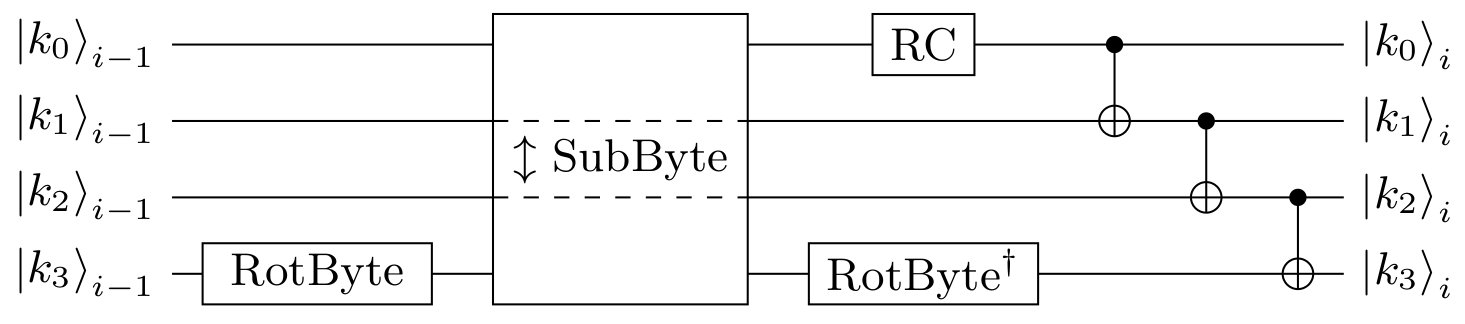
\includegraphics[width=\linewidth]{aes/aeske.png}
    \caption{AES-128 key expansion \cite{aeslowmc}}
    \label{fig:aeske}
\end{figure}

$\ket{k_j}_i$ represent the $j^{th}$ word (4 bytes) of the $i^{th}$ round key. First $\ket{k_3}_{i-1}$ (last word) is rotated and then passed through AES Sbox. The output of this operation is collected at the first word i.e. the output is XORed with $\ket{k_0}_{i-1}$. The result is then added with a round constant for that round. The next steps involve XORing with other words of $(i-1)^{th}$ round key to obtaining words of $i^{th}$ round key which is performed using CNOT gates. The dotted lines in the Sbox represent that the corresponding wires have not been used in Sbox operation.

\subsection{QAES-128 circuit}
Figure \ref{fig:aesfull} shows the QAES circuit. Each wire represents 4 words (128 qubits). $\ket{k}$ represents the master key and $\key{m}$ represents the message. BS is Sbox, SR is shift rows and MC is mix column. Here we have used an in-place version of mix columns.

\begin{figure}[h!]
    \centering
    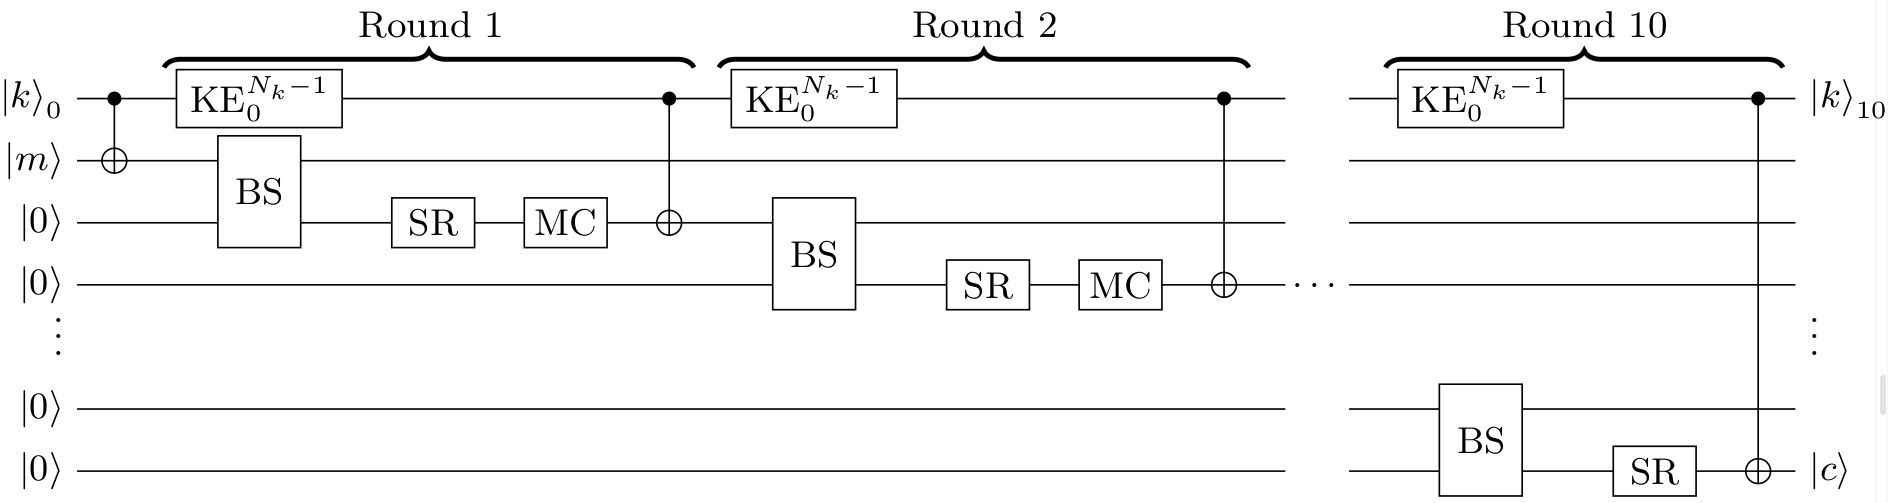
\includegraphics[width=\linewidth]{aes/aesfull.png}
    \caption{QAES-128 \cite{aeslowmc}}
    \label{fig:aesfull}
\end{figure}

Table \ref{tab:aescost} shows the cost of QAES-128 for both variants of mix columns. The in-place version of the mix column has lower DW-cost and G-cost compared to \cite{aesmc} version. 


\begin{center}
\begin{table}[h!]
    \centering
    \begin{tabular}{ |c|c|c|c|c|c|c|c|c| } 
     \hline
     MC & CNOT & Clifford & T & M & T-depth & full depth & width & DW \\ \hline
    QAES-128 In place  & 2,91,150& 83,116&54,400&13,600&120&2,827&1,785&50,46,195 \\ \hline
     QAES-128 \cite{aesmc} &2,93,730&83,236&54,400&13,600&120&2,094&2,937&61,50,078   \\ \hline
    \end{tabular}
    \caption{QAES-128 cost of both variants of mix columns}
    \label{tab:aescost}
\end{table}
\end{center}

\subsection{Grover's Attack}
Figure \ref{fig:aesgrov} shows the Grover Oracle for 1 iteration. FwAES implies the forward AES which outputs the ciphertexts without cleaning the qubits. FwAES$\dagger$ circuit is the reversible operation of FwAES which cleans the qubits. The attack requires $r = 2$ plaintext-ciphertext pair for finding the unique key. The oracles cost is shown in Table \ref{tab:aesgrovcost}

\begin{figure}[h!]
    \centering
    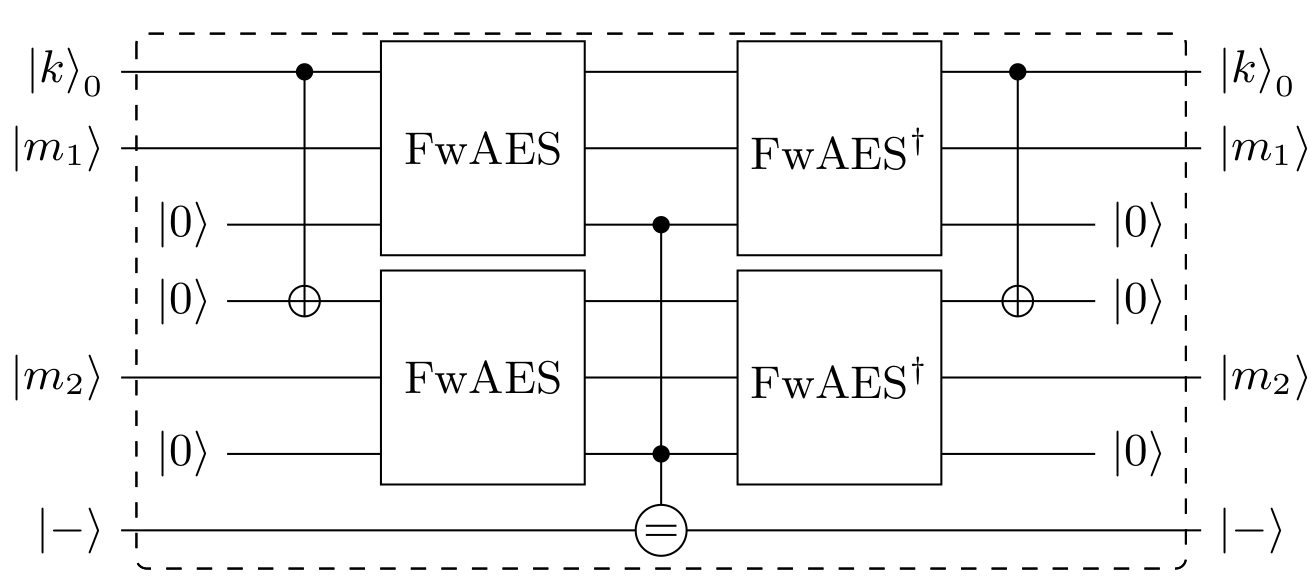
\includegraphics[width=\linewidth]{aes/aesrov.png}
    \caption{Grover's Attack on QAES-128 \cite{aeslowmc}}
    \label{fig:aesgrov}
\end{figure}

\begin{center}
\begin{table}[h!]
    \centering
    \begin{tabular}{ |c|c|c|c|c|c|c|c|c| } 
     \hline
     MC & CNOT & Clifford & T & M & T-depth & full depth & width & DW \\ \hline
    QAES-128 In place  & 5,85,051&1,69,184&1,09,820&27,455&121&2,815&3,329&93,71,135 \\ \hline
     QAES-128 \cite{aesmc} & 5,89,643&1,68,288&1,09,820&27,455&121&2,096&5,633&1,18,06,768  \\ \hline
    \end{tabular}
    \caption{QAES-128 Grover's Oracle cost of both variants of mix columns (r=2)}
    \label{tab:aesgrovcost}
\end{table}
\end{center}

\subsubsection{Cost Estimates}
With the help of Table \ref{tab:aescost} and the equations \ref{eq:D},\ref{eq:gcost}, and \ref{eq:DW} we can calculate the cost estimates for Grover's Attack without depth restriction. Using equations \ref{eq:S}, \ref{eq:G}, and \ref{eq:DW2} we can calculate the cost estimates for Grover's Attack with depth restriction.

Let's calculate the cost estimates of Grover's Attack on QAES-128 in place with r = 2 with and without depth constraint. The total gate cost $G_G$ is the sum of all the gates shown in Table \ref{tab:aescost} i.e.
\begin{equation*}
    \begin{aligned}
        G_G &= 5,85,051 + 1,69,184 + 1,09,820 + 27,455 = 8,91,510 \approx 1.7 \times 2^{19} \\
        G_D &= 2,815 \approx 1.37 \times 2^{11} \\
        G_W &= 3,329 \approx 1.62 \times 2^{11}
    \end{aligned}
\end{equation*}
Therefore the cost estimates without depth constraints keeping $S = 1$ is:
\begin{equation*}
    \begin{aligned}
        D &\approx 1.37 \times 2^{11} \times 2^{64} = 1.37 \times 2^{75} \\
        G &\approx 1.7 \times 2^{19} \times 2^{64} = 1.7 \times 2^{83} \\
        DW &\approx 1.37\times 2^{11} \times 1.62 \times 2^{11} \times 2^{64} \approx 1.1 \times 2^{87}
    \end{aligned}
\end{equation*}

Similarly, the cost estimates with depth constraint of $2^{40}$ are:
\begin{equation*}
    \begin{aligned}
        S &\approx 2^{128}\times 1.37^2 \times 2^{22} \times 2^{-80} \approx 1.87 \times 2^{70} \\
        G &\approx 2^{128} \times 1.37 \times 2^{11} \times 1.7 \times 2^{19} \times 2^{-40} \approx 1.16 \times 2^{119} \\
        DW &\approx 2^{128} \times 1.37^2 \times 2^{22} \times 1.62 \times 2^{11} \times 2^{-40} \approx 1.52 \times 2^{122}
    \end{aligned} 
\end{equation*}

NIST\cite{nist} has proposed a maximum of $2^{170}/$MAXDEPTH quantum gates for AES-128 but this does not take into account the effects of parallelization. For MAXDEPTH = $2^{40}$, \cite{nist} has bounded the count of quantum gates by $2^{170}/2^{40} = 2^{130}$. From the above calculation of G-cost we can see that the number of gates required by AES-128 is much less after parallelization ($2^{119}$).

\section{Conclusion}\label{sec:con}
Applications of Grover's search algorithm in Quantum cryptanalysis are studied in this paper. We briefly studied hardware and software-friendly ciphers. The Quantum circuit for SAES was modeled and then the quantum resources were optimized. As a result, the quantum architecture is not a barrier to a quantum adversary carrying out any potential quantum attack. We designed a Quantum circuit for SIMON and PRESENT ciphers which are hardware friendly with a minimal number of qubits. We then discussed the parallelization of Grover's algorithm and its cost estimates which are used in modeling the quantum circuit and estimating the quantum resources for AES-128. AES-128 was studied with and without depth constraints under the rules proposed by NIST \cite{nist}.

We implemented SAES and QSAES in python using Qiskit\cite{Qiskit} and libquantum\cite{libquantum} to verify the results. We were unable to run a successful Grover's Attack as it was time-consuming. It seems that current frameworks are not yet optimized for running a full Grover's Attack to find a unique key using minimum resources and have a scope of optimization. libquantum written in C has issues when running codes across different machines. The code and obtained results are open-sourced \cite{Gopal}.



\printbibliography[title={References}] 

%%%% 8. BILBIOGRAPHY %%%%

% \bibliographystyle{alpha}
% \bibliography{abbrev3,crypto,biblio}
%%%% NOTES
% - Download abbrev3.bib and crypto.bib from https://cryptobib.di.ens.fr/
% - Use bilbio.bib for additional references not in the cryptobib database.
%   If possible, take them from DBLP.




\end{document}